%
% 修士学位請求論文(副・正)テンプレート
% MasterThesisSample.tex
% By KASHINA, Yuki (EM-14003)
%
\documentclass{MasterThesis}
%\documentclass[fleqn]{MasterThesis} %数式を左寄せ


%%%%%%%%%%%%%%%%%%%%%%%%%%%%%%%%%%%%%%%%%%
% ユーザ任意のパッケージ
%%%%%%%%%%%%%%%%%%%%%%%%%%%%%%%%%%%%%%%%%%
%\usepackage{booktabs}
%\usepackage{multirow}
\usepackage[dvipdfmx]{xcolor}
\usepackage{otf}


%%%%%%%%%%%%%%%%%%%%%%%%%%%%%%%%%%%%%%%%%%
% マクロ
%%%%%%%%%%%%%%%%%%%%%%%%%%%%%%%%%%%%%%%%%%
%<local definition>
\newcommand{\texcmd}[1]{\texttt{\textbackslash{}#1}}

\usepackage{setspace}
\def\commentary#1{\raisebox{\baselineskip}{\parbox{0.8\textwidth}{\begin{spacing}{0.8}#1\end{spacing}}}\vspace{.42\baselineskip}\endgraf}
%</local definition>


%%%%%%%%%%%%%%%%%%%%%%%%%%%%%%%%%%%%%%%%%%
% ルートパス
%%%%%%%%%%%%%%%%%%%%%%%%%%%%%%%%%%%%%%%%%%
\graphicspath{{figure/}}
\tablepath{{table/}}


%%%%%%%%%%%%%%%%%%%%%%%%%%%%%%%%%%%%%%%%%%
% 行間調整
%%%%%%%%%%%%%%%%%%%%%%%%%%%%%%%%%%%%%%%%%%
\renewcommand{\baselinestretch}{1.0}


%%%%%%%%%%%%%%%%%%%%%%%%%%%%%%%%%%%%%%%%%%
% 図表キャプションの接頭辞
%%%%%%%%%%%%%%%%%%%%%%%%%%%%%%%%%%%%%%%%%%
%\renewcommand{\jfigurename}{図}
%\renewcommand{\jtablename}{表}
%\renewcommand{\efigurename}{Fig.~}
%\renewcommand{\etablename}{Table~}


%%%%%%%%%%%%%%%%%%%%%%%%%%%%%%%%%%%%%%%%%%
% フォントサイズ
%%%%%%%%%%%%%%%%%%%%%%%%%%%%%%%%%%%%%%%%%%
%%% 英文タイトル
%\renewcommand{\etitlefontsize}{\fontsize{21pt}{21pt}}
\renewcommand{\etitlefontsize}{\fontsize{14pt}{14pt}}

%%% 本文
%\renewcommand{\mainfontsize}{\fontsize{14pt}{25pt}}
\renewcommand{\mainfontsize}{\fontsize{12pt}{21pt}}

%%% キャプション
\renewcommand{\captionfontsize}{\fontsize{11pt}{14pt}}


%%%%%%%%%%%%%%%%%%%%%%%%%%%%%%%%%%%%%%%%%%
% 書誌情報
%%%%%%%%%%%%%%%%%%%%%%%%%%%%%%%%%%%%%%%%%%
%%% 和文タイトル
% \newlineで改行,数式やコマンド,クォートは{}でグルーピング
% \jtitle{体験情報に基づくLies-Bias型観光支援システム}{}
\jtitle{既訪問スポットと検索結果の対応付けに基づく観光地検索システムの説明性向上手法}{}

%%% 英語タイトル・サブタイトル
% \etitle{ユーザの訪問情報を用いた観光支援システム}{}

%%% 所属専攻 //工学研究科は不要
\affiliate{情報学専攻}

%%% 氏名・学籍番号 //\ruby{漢字}{かん|じ}, 性名間に半角空白を挿入
\author{\ruby{潘}{はん}~\ruby{健太}{けん|た}}

%%% 指導教官名・指導教官役職 //姓名間に半角空白を挿入
\supervisor{北山~大輔}{准教授}

%%% 修了年月(西暦) //全角を推奨
\ptdate{2020}{3}

%%% 前文のタイトル
\abstractname{要旨}{Abstract}

%%% 目次の有効化
\toctrue

%%% 図目次の有効化
\loftrue

%%% 表目次の有効化
\lottrue

%%% 索引の有効化
%\makeindex

%%% 研究室内部資料セクション(付録)の有効化
%\domestictrue



%%%%%%%%%%%%%%%%%%%%%%%%%%%%%%%%%%%%%%%%%%
% 書誌情報の設定終了
%%%%%%%%%%%%%%%%%%%%%%%%%%%%%%%%%%%%%%%%%%
\eom



%%%%%%%%%%%%%%%%%%%%%%%%%%%%%%%%%%%%%%%%%%
% 前文(和文)
\jabstract
%%%%%%%%%%%%%%%%%%%%%%%%%%%%%%%%%%%%%%%%%%
近年,ユーザは観光旅行をする前にWeb上の情報やガイドブックを活用して計画を立てることが多くなっていると考えられる.
旅行計画を立てるためには,まず訪問したいエリアを決定する.
その後,観光スポット検索サイトやガイドブックの観光スポット情報を調べて観光スポットを決定する.
その際,目的とする観光スポットに関する概要やアクセスするための方法などの情報を集める.

Web上の情報に関して,観光スポットに関する総合的な情報が掲載された公式サイト,過去にそこを訪れた観光者による旅行記ブログサイト,そして,評価が記載されたレビューサイトなどのさまざまなサイトがある.
しかしながら,種々のサイトが混在しており,膨大な情報から自分の嗜好に合う観光スポットの情報を得ることは簡単ではない.
目的の情報を収集するためには手動で閲覧し取捨選択しなければならない.
ユーザの意思決定のための材料の1つとして,観光スポット検索サイトがある.観光スポット検索サイトには特定の観光スポットを訪問したことのあるユーザがレビューを投稿しており,観光スポットに関する情報が豊富にある.
観光スポット検索サイトに掲載された情報を基に,利用者(ユーザ)は自身の嗜好や目的に合致した特徴を持つ対象観光スポットを検索する.
多くの観光スポット検索サイトでは,対象観光スポットに付与されるメタデータを利用した以下のような検索方法が提供されている.
\begin{itemize}
    \item ユーザが指定したタグを持つ対象観光スポット
    \item 評価点などの数値メタデータに基づく並び替え
    \item 入力単語(クエリ)を概要文中に含むオブジェクトの検索
\end{itemize}

しかし,これらのメタデータを用いた検索方法だけではユーザが指定された範囲内しか検索できない.
たとえば,対象観光スポットを実際に利用することでユーザが得られる印象・感情・体験などを表す特徴に基づき,対象観光スポットを検索したい場合などが該当する.
また,検索できたとしても訪問したいエリア内には数多くの観光スポットが検索結果として表示される.
ユーザは多くの場合,検索エリアに関する事前知識がないため,検索された多数の観光スポットからどの観光スポットの説明やレビューを読むべきか効率的に判断することは困難であり,自身の要求に合う観光スポットを見つけることは容易ではない.

一方,ガイドブックは,Web上の情報に比べて整理されており,有名な観光スポットや流行のものに焦点を当て,そのスポットの料金や見どころ,そして食べ物などが掲載されている.
また,ガイドブックも近年は電子化されており,技術的には検索可能である.
しかしながら,ある観光スポットについて,複数のガイドブックが取り上げることもあり,行き方の比較検討をするためにそれらを読むのは労力を必要とする.
そのため,Web上の情報と同じ問題が起こり得る.

そこで本研究では,観光地検索システムの検索結果である観光スポットを効率的に理解するために,ユーザが訪問したことがある観光スポット(既訪問スポット)を使って説明性を向上する手法を開発する.
本手法を開発するにあたり2つの課題を解決する必要がある.

\begin{enumerate}
\item 観光スポット間の対応付け

第1の課題として,既訪問スポットと検索結果スポットをどのように対応付けると説明として効果的なのか明らかではないことがある.
ある観光スポットに対応する観光スポットを判定する手法として,レビューやカテゴリが類似したコンテンツであるという観点で判定する方法が一般的である.
カテゴリなどのメタデータが類似する対応付けの場合には,大まかな利用目的レベルでの説明が可能であると考えられる.
レビューが類似するという場合には,より細かい体験のレベルでの説明が可能となると考える.
このように対応付けの方法によって,その説明性も変化すると考えられる.
また,本研究における観光スポットの対応付けに関して,ユーザによって,その強調するべき特徴が変化することがあり得る.
たとえば,日本の有名な観光スポットを履歴に持つユーザにとっての「東京都庁舍展望台」と「金閣寺」について考える.
このとき,このユーザにとっての「金閣寺」の特徴は,お寺,金色,京都などである.
また,「東京都庁舍展望台」の特徴は,展望,夜景,建物,新宿などが考えられる.
一方,京都の寺院を履歴に持つユーザにとっての「金閣寺」と「清水寺」について考える.
このとき,同じ「金閣寺」でもお寺や京都などは特徴にはならず,このユーザにとっての「金閣寺」の特徴は,金色,金箔,輝きなどとなる.
また,「清水寺」の特徴は,舞台や一望などである.
このように強調すべき点が異なる特徴を相対的特徴と定義する.
前述の2つに加え,相対的特徴による類似度という詳細なレベルでの対応付けを行い,比較することで,説明に適した対応付け手法を明らかにする.

\item 地図上における観光スポットの対応関係の可視化

第2の課題は,数多くあるユーザの過去の訪問先と検索結果をどのように提示すると,説明として適切であるか明らかではないことである.
まず,地理的情報の可視化と意味的な関係を同時に可視化することを考える.
地理情報の可視化としては,抽出した情報を地図上にマッピングするのが一般的である.
また,意味的な関係性の可視化として,グラフモデル上でオブジェクト間のつながりを関連度で表現することが多い.
観光スポット間の意味的な対応関係を可視化するために,検索結果スポットは地図上で実在する座標に固定し,既訪問スポットを関連度に基づいて適切に配置することが妥当であると考える.
そこで,ある検索結果スポットに対して,入力した既訪問スポットがどのような関係にあるのか地図上で,一目で把握できるように,既訪問スポットと検索結果スポットの対応関係を可視化する手法を提案し,一般的な表形式や表示情報を増加させた形式と比較する.
このことにより,説明として適切な可視化方法を明らかにする.
\end{enumerate}

各課題についての取り組みの詳細を説明する.
1.の観光スポットの間の対応付けについては以下に記す.
ユーザがいままで体験したことがあり,かつ気に入った観光スポットを利用し,訪問したいエリア内の観光スポットに対して関連付けすることで,手軽に観光情報を理解する説明性向上手法を提案する.
まず,ユーザは体験履歴の中でいままで訪れたことがある,かつ気に入った観光スポットを入力する.
次に,これから行ってみたい都道府県やエリアを入力する.
これらの入力に対し,観光スポット検索サイトの観光スポットのレビューデータを使ってユーザの体験履歴と検索結果を対応付ける.
すなわち,ユーザの未知な観光スポットに対する理解を支援するため,すでに訪問したことがある観光スポットの特徴を用いて,未訪問エリアの観光スポットを説明するために対応付けを行う.
この考え方は,ユーザが以前に経験した物事を現在の物事に適用する一種の類推であるといえる.
既知の知識(ベースと呼ぶ)から概念(ターゲットと呼ぶ)を獲得するときに類推思考が働くとされる.

具体的な対応付け手法について説明する.
ある検索結果スポットの特徴ベクトルに最も類似度が高い既訪問スポットを対応付ける.
類似度計算には,コサイン尺度を用いる.
観光スポットの対応関係を示すだけでは,どのような点で対応するのかを理解するのは難しい.
そこで,検索結果スポットと既訪問スポットの関係性を表すキーワードをユーザに提示する.
キーワード抽出手順は,TF-IDF法を使って対象となる既訪問スポットと検索結果スポットの特徴語とTF-IDF値を求める.
2つのスポットに共通する特徴語のTF-IDF値の調和平均を用いて,対応付けしたスポットの説明可能なキーワードとして抽出する.
また,相対的特徴を定義し,通常用いられる特徴ベクトルでの対応付けに加え,本研究では,この効果も明らかにする.

観光スポット間の対応付けを評価するために,対応関係を表す特徴語抽出評価,観光スポットの対応付けに関する評価,検索結果スポット説明の有効性評価の3つの評価実験を行った.
対応関係を表す特徴語抽出評価について,提案手法である調和平均を用いて特徴語を抽出する手法は,算術平均法と乗算法より観光スポット間の隠れた関係を表現することが可能かつ,無関係な特徴語を抽出しにくいことが確認できた.
観光スポットの対応付けに関する評価について,相対的特徴ベクトルを用いて対応付けするのは,メタデータ法と分散表現法より詳細な情報をユーザに提示することができることを明らかにした.
しかし,相対的特徴ベクトルでは,ユーザに提示する関連するスポットについての意外性はあるが,無関係に見える対応付けをする問題点があることがわかった.
検索結果スポット説明の有効性評価について,提案手法では検索結果スポット名,対応する既訪問スポット名と対応関係を説明するための特徴語を提示しているに対し,検索結果スポット名のみとの比較を行った結果,提案手法の方がユーザにとって観光スポット間の関連性が連想しやすく,旅行を計画するのに有用であることがわかった.

2.の地図上における観光スポットの対応関係の可視化については以下に記す.
地図上で既訪問スポットと検索結果スポットの対応関係と特徴語を可視化することで,ユーザの検索結果スポットに対する理解を容易化することを目指す.
そのために,ある検索結果スポットに対して,入力した既訪問スポットがどのような関係にあるのか,地図上で一目で把握できることが望ましい.
ユーザは地図上で観光スポットを検索しているものとし,まず,地図上の実際にスポットが存在する座標に検索結果スポットを配置する.
次に,既訪問スポットの位置を決定する.
これは検索結果スポットとの対応関係によって変化し,検索結果スポットとの類似度が高いと近く,類似度が低いと遠くなるように配置することで,意味的な位置関係を表現する.

観光スポットの対応関係の可視化を評価するために,分散表現ベクトルによる対応関係を用いた実験と相対的特徴ベクトルによる対応関係を用いた実験を行った.
2種類のベクトルによるそれぞれの評価実験に対して,検索対象のスポットと既訪問スポットの関連度を全体的な位置関係で表現している$Position\_Map$,位置関係による提示に加えて線の色を使って表現している$Line\_Map$,位置関係や線は用いずに$Line\_Map$で表現していたすべての情報を表形式で表現している$Table\_Map$の3つの提示手法を比較することで評価を行った.
結果,分散表現ベクトルによる対応関係の可視化に関して$Position\_Map$がユーザにとってもっとも理解しやすいことがわかった.
一方,相対的特徴ベクトルによる対応関係の可視化に関して$Table\_Map$がユーザにとってもっとも理解しやすいことがわかった.
このことより,分散表現ベクトルを使って観光スポットの特徴抽出と対応付けを行うことによって,観光スポット間の違いを直感的に地図上に表示することができたため,一目で観光スポットの対応関係を把握することができることを示した.

%%%%%%%%%%%%%%%%%%%%%%%%%%%%%%%%%%%%%%%%%%
% 本文の開始
%%%%%%%%%%%%%%%%%%%%%%%%%%%%%%%%%%%%%%%%%%
\main

%%%%%%%%%%%%%%%%%%%%%%%%%%%%%%%%%%%%%%%%%%
\chapter{序論}
%%%%%%%%%%%%%%%%%%%%%%%%%%%%%%%%%%%%%%%%%%
近年,ユーザは観光旅行をする前にWeb上の情報やガイドブックを活用して計画を立てることが多くなっていると考えられる.
旅行計画を立てるためには,まず訪問したいエリアを決定する.
その後,観光スポット検索サイトやガイドブックの観光スポット情報を調べて観光スポットを決定する.
その際,目的とする観光スポットに関する概要やアクセスするための方法などの情報を集める.

Web上の情報に関して,観光スポットに関する総合的な情報が掲載された公式サイト,過去にそこを訪れた観光者による旅行記ブログサイト,そして,評価が記載されたレビューサイトなどのさまざまなサイトがある.
しかしながら,種々のサイトが混在しており,膨大な情報から自分の嗜好に合う観光スポットの情報を得ることは簡単ではない.

ユーザの意思決定のための材料の1つとして,るるぶトラベル\footnote{https://www.rurubu.travel/},Tripadvisor\footnote{https://www.tripadvisor.com/}やじゃらん\footnote{https://www.jalan.net/kankou/}などの観光スポット検索サイトがある.観光スポット検索サイトには特定の観光スポットを訪問したことのあるユーザがレビューを投稿しており,観光スポットに関する情報が豊富にある.
観光スポット検索サイト上で観光スポットに付与される情報の例\footnote{https://www.jalan.net/kankou/130000/?screenId=OUW2201}を図\ref{fig:レビューサイト上で観光スポットに付与される情報例}に示す.
なお,これらの情報のうちユーザレビュー以外の情報(概要文・タグ・評価点など)はメタデータと呼ばれる.
\begin{figure}[t]
    \centering
    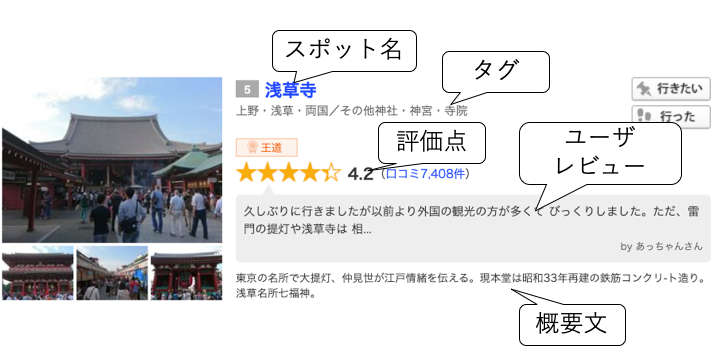
\includegraphics[width=0.9\textwidth]{./figure/spot_info.png}
    \caption{レビューサイト上で観光スポットに付与される情報例}
    \label{fig:レビューサイト上で観光スポットに付与される情報例}
\end{figure}

観光スポット検索サイトに掲載された情報を基に,利用者(ユーザ)は自身の嗜好や目的に合致した特徴を持つ対象観光スポットを検索する.
多くの観光スポット検索サイトでは,対象観光スポットに付与されるメタデータを利用した以下のような検索方法が提供されている.

\begin{itemize}
    \item ユーザが指定したタグを持つ対象観光スポット
    \item 評価点などの数値メタデータに基づく並び替え
    \item 入力単語(クエリ)を概要文中に含むオブジェクトの検索
\end{itemize}

% しかし,これらのメタデータを用いた検索方法だけでは検索が困難な場合もある.
しかし,これらのメタデータを用いた検索方法だけではユーザが指定された範囲内しか検索できない.
たとえば,対象観光スポットを実際に利用することでユーザが得られる印象・感情・体験などを表す特徴に基づき対象観光スポットを検索したい場合などが該当する.
また,検索できたとしても訪問したいエリア内には数多くの観光スポットが検索結果として表示される.
ユーザは多くの場合,検索エリアに関する事前知識がないため,検索された多数の観光スポットからどの観光スポットの説明やレビューを読むべきか効率的に判断することは困難であり,自身の要求に合う観光スポットを見つけることは容易ではない.

一方,ガイドブックは,Web上の情報に比べて整理されており,有名な観光スポットや流行のものに焦点を当て,そのスポットの料金や見どころ,そして食べ物などが掲載されている.
また,ガイドブックも近年は電子化されており,技術的には検索可能である.
ある観光スポットについて,複数のガイドブックが取り上げることもあり,行き方の比較検討をするためにそれらを読むのは労力を必要とする.
そのため,Web上の情報と同じ問題が起こり得る.

そこで,本研究では,観光地検索システムの検索結果である観光スポットを効率的に理解するために,ユーザが訪問したことがある観光スポットを使って説明性を向上する手法を開発する.
本手法を開発するにあたり2つの課題を解決する必要がある.

\begin{enumerate}
\item 観光スポット間の対応付け

第1の課題として,既訪問スポットと検索結果スポットをどのように対応付けると説明として効果的なのか明らかではないことがある.
ある観光スポットに対応する観光スポットを判定する手法として,レビューやカテゴリが類似したコンテンツであるという観点で判定する方法が一般的である.
カテゴリなどのメタデータが類似する対応付けの場合には,大まかな利用目的レベルでの説明が可能であると考えられる.
レビューが類似するという場合には,より細かい体験のレベルでの説明が可能となると考える.
このように対応付けの方法によって,その説明性も変化すると考えられるが,どのような対応付けを行うと,説明として,どのような効果が得られるのかは明らかではない.
そこで,本研究では,前述の2つに,さらに,相対的な特徴による類似という,より詳細なレベルでの対応付けを加え,比較することで,説明に適した対応付け方法を明らかにする.

相対的な特徴に関して,同じスポットでも,ユーザによって,その強調するべき特徴が変化することがあり得る.
たとえば,日本の有名な観光スポットを履歴に持つユーザにとっての「東京都庁舍展望台」と「金閣寺」について考える.
このとき,このユーザにとっての「金閣寺」の特徴は,お寺,金色,京都などである.
また,「東京都庁舍展望台」の特徴は,展望,夜景,建物,新宿などが考えられる.
一方,京都の寺院を履歴に持つユーザにとっての「金閣寺」と「清水寺」について考える.
このとき,同じ「金閣寺」でもお寺や京都などは特徴にはならず,このユーザにとっての「金閣寺」の特徴は,金色,金箔,輝きなどとなる.
また,「清水寺」の特徴は,舞台や一望などである.
このように強調すべき点が異なる特徴を相対的特徴と定義する.
前述の2つに加え,相対的特徴による類似度という詳細なレベルでの対応付けを行い,比較することで,説明に適した対応付け手法を明らかにする.

\item 地図上における観光スポットの対応関係の可視化

第2の課題は,数多くあるユーザの過去の訪問先と検索結果をどのように提示すると,説明として適切であるか明らかではないことである.
まず,地理的情報の可視化と意味的な関係を同時に可視化することを考える.
地理情報の可視化としては,抽出した情報を地図上にマッピングするのが一般的である.
また,意味的な関係性の可視化として,グラフモデル上でオブジェクト間のつながりを関連度で表現することが多い.
観光スポット間の意味的な対応関係を可視化するために,検索結果スポットは地図上で実在する座標に固定し,既訪問スポットを関連度に基づいて適切に配置することが妥当であると考える.
そこで,ある検索結果スポットに対して,入力した既訪問スポットがどのような関係にあるのか地図上で,一目で把握できるように,既訪問スポットと検索結果スポットの対応関係を可視化する手法を提案し,一般的な表形式や表示情報を増加させた形式と比較する.
このことにより,説明として適切な可視化方法を明らかにする.
\end{enumerate}

以下に本論文の構成を示す.
ます,2章で本研究のアプローチについて述べる.
ここでは観光支援システムのアルゴリズムと関連研究について述べる.
この観光支援システムのための2つの観点に基づく各手法は3章と4章で述べる.
3章では,ユーザの既訪問スポットの位置付けに基づく検索結果スポットの説明手法について述べる.
4章では,地図上における検索結果スポットの説明向上のための観光スポットの対応付け可視化手法について述べる.
5章では,まとめと今後の課題を述べる.


%%%%%%%%%%%%%%%%%%%%%%%%%%%%%%%%%%%%%%%%%%
\chapter{本研究のアプローチ}
%%%%%%%%%%%%%%%%%%%%%%%%%%%%%%%%%%%%%%%%%%
\section{説明性向上手法}
一般的な観光スポット検索システムは,訪問したいカテゴリやエリアを入力して検索を行い,検索結果の観光スポットをリスト形式でユーザに表示する.
また,地図上にプロットして表示する機能を備えているものもある.
地図上での検索としては,Google Mapなどの地図サイトで「観光」をキーワードに検索することも可能である.
このように,検索結果の一貫性や網羅性は高い.
図\ref{fig:観光スポット検索システムの例}の左側はTripAdvisorによる西新宿エリアの地図表示であり,観光スポットが地図上にプロットされた検索結果が表示される.
一方,検索結果の詳細は,そのスポットをクリックして詳細情報を表示するまでわからない.
このとき地図上に,自身が訪れたことがあるスポットと検索結果の関係がわかる情報が表示されていれば,詳細情報を確認する前に,そのスポットについて知ることができると考えた.
このような,検索結果自体が理解しやすくなることを説明性の向上と定義する.
図\ref{fig:観光スポット検索システムの例}の右側は左側の検索結果に説明性向上を施したものである.
図\ref{fig:観光スポット検索システムの例}の左側は「東京都庁展望室」などの検索結果スポットのみ地図上で表示されていることに対し,右側は検索結果スポットと既訪問スポットが表示されている.
この例では,ユーザが過去に「梅田スカイビル」,「住吉大社」に訪ねていることを想定している.
図\ref{fig:観光スポット検索システムの例}の右側の図から一目で,「梅田スカイビル」は「東京都庁展望室」との関連性が強く,「住吉大社」は関連性が低いことがわかる.

\begin{figure}[t]
    \centering
    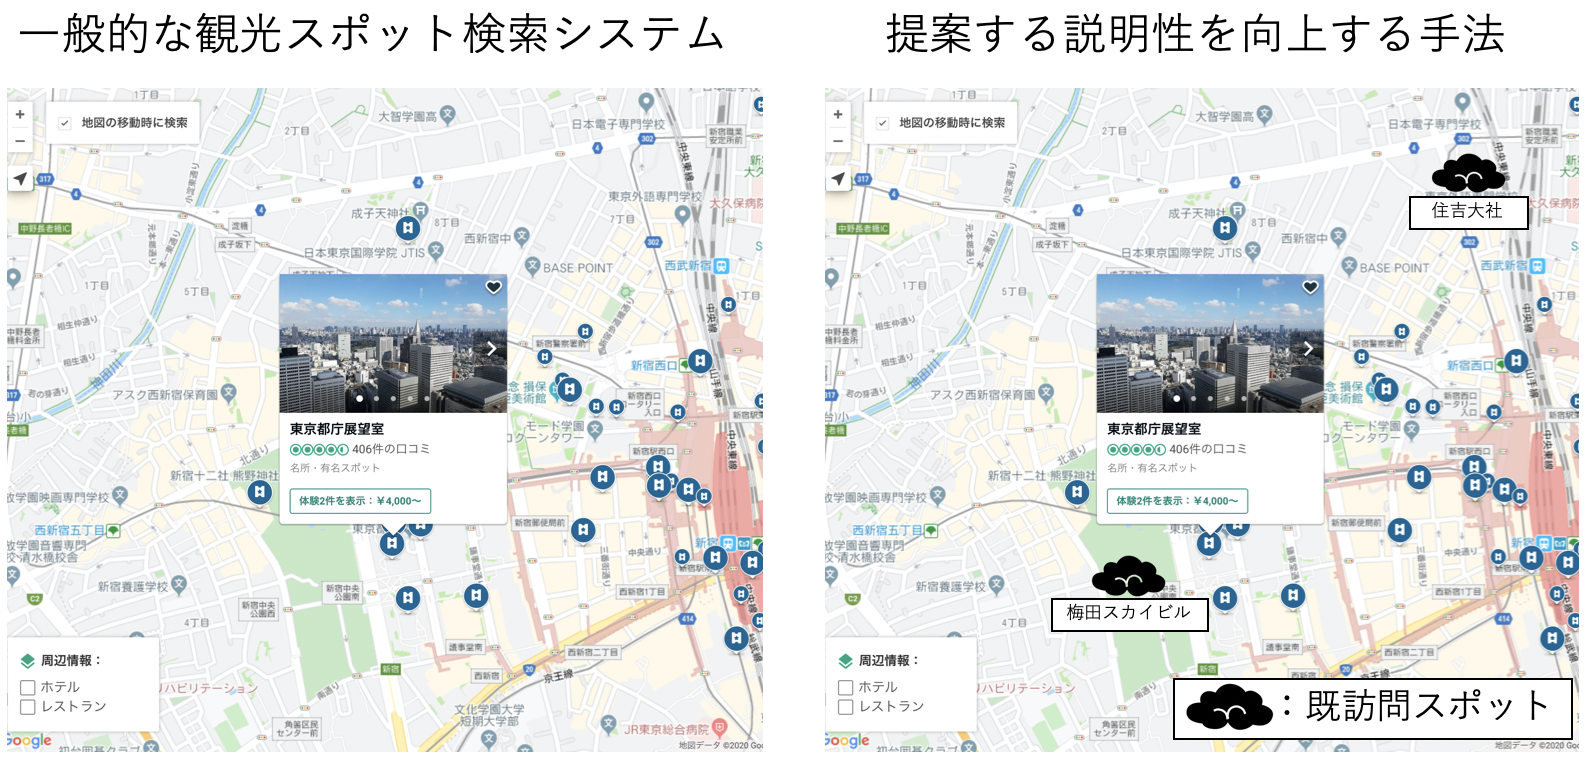
\includegraphics[width=0.9\textwidth]{./figure/image.png}
    \caption{一般的な観光スポット検索システムと提案する説明性を向上する手法}
    \label{fig:観光スポット検索システムの例}
\end{figure}

観光支援システムの1つに,求める観光スポット情報を発見するために観光スポットの理解をしやすくすることが考えられる.
観光情報収集までの過程を効率化することで,ユーザの旅行計画の敷居は下がり,訪れたことない観光スポットの理解の向上も望める.
本研究では,ユーザがいままで体験したことがあり,かつ気に入った観光スポットを利用し,訪問したいエリア内の観光スポットに対して関連付けすることで,手軽に観光情報を理解する説明性向上手法を提案する.
\begin{figure}[t]
    \centering
    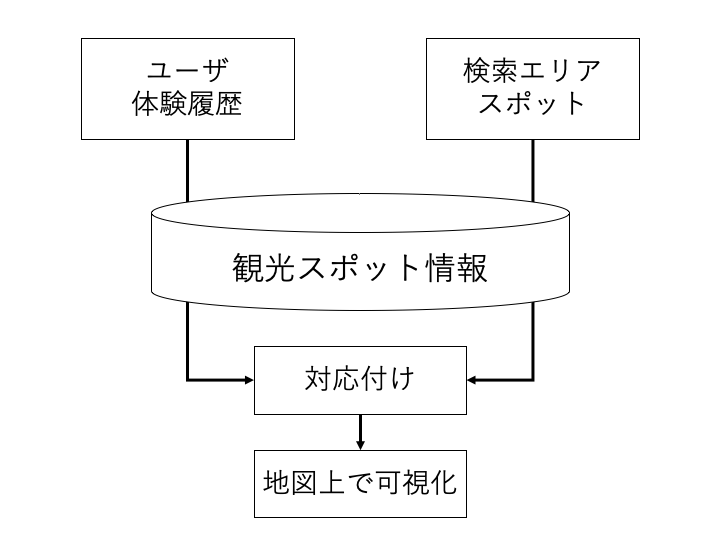
\includegraphics[width=0.9\textwidth]{./figure/system_fig.png}
    \caption{観光地検索システムの説明性向上手法}
    \label{fig:観光地検索システムの}
\end{figure}

観光地検索システムの説明性向上手法の流れを図\ref{fig:観光地検索システムの}に沿って説明する.
まず,ユーザは体験履歴の中でいままで訪れたことがあり,かつ気に入った観光スポットを入力する.
次に,これから行ってみたい都道府県やエリアを入力する.
これらの入力に対し,ユーザの体験履歴と検索結果を対応付ける.
すなわち,ユーザの未知な観光スポットに対する理解を支援するため,すでに訪問したことがある観光スポットの特徴を用いて,未訪問エリアの観光スポットを説明するための対応付けを行う.

対応付けを行うために既訪問スポットと検索結果スポットの特徴ベクトルを求める必要がある.
特徴ベクトルを求める代表的な手法として,TF-IDF法\cite{TF,IDF}やParagraph Vectorモデル\cite{Le}(Doc2Vec)などがある.
対応付け部分において,本研究では,基本的には従来手法をそのまま用いる.
この部分における本研究の貢献は,ユーザの体験履歴を用いたスポットの説明としての各種対応付け手法の特性を明らかにすることにある.
また,予備実験において,TF-IDF法とParagraph Vectorモデルを用いて特徴ベクトルを計算し,類似度を使ってスポット間の対応付けを行なった.
その予備実験の結果より,TF-IDF法とParagraph Vectorモデルの対応付けでは,既訪問スポットと検索結果スポットはほぼ同じ対応付けとなることがわかった.
よって,本研究では,類語を含めて対応付けできることが期待できる手法のParagraph Vectorモデルを用いる.

対応付けを行ったあと,ユーザに検索結果スポットを説明するための観光スポット特徴語を抽出する.
最後に,地図上で既訪問スポットと検索結果スポットの対応関係と特徴語を可視化することで,ユーザが検索結果スポットに対する理解を容易化することを目指す.

%%%%%%%%%%%%%%%%%%%
\section{関連研究}
本研究では,ユーザの体験履歴の中のレビューを分析し,地図上で対応関係を可視化して観光情報を理解する説明性向上手法を提案する.
本研究の特徴は,体験履歴を検索結果の説明性向上に用いることと,地図上で意味的な関係性を可視化することである.
そこで,従来のユーザの体験履歴を用いた検索や推薦に関する研究を紹介することでアプローチの違いを述べる.
次に,地理的な情報の可視化と意味的な関係の可視化に関する研究を紹介することで可視化の問題を整理する.
%%%%%%%%%%%
\subsection{体験履歴による検索や推薦システムに関する研究}
本研究では,ユーザの体験履歴を検索結果の個人化した説明に用いる.
そこで,検索や推薦システムでの体験履歴の一般的な用いられ方を紹介することでアプローチの違いを説明する.

まず,体験履歴は個人化のために用いられることが多い.
倉島ら\cite{Kurashima}は,Flickrに投稿された写真のジオタグ情報を人々の旅行履歴として利用した旅行ルート推薦手法を提案した.この手法では,ユーザの現在地から行きやすい場所とユーザの興味に合致した場所に移動しやすいと仮定し,行動モデルを生成している.
ユーザのジオタグ付き写真集合は,時間情報でソートすると個人の旅行履歴とみなすことができると考え,ジオタグ情報を利用してユーザの行動モデルを生成している.
Chengら\cite{Cheng}は,自由に利用できるコミュニティ投稿の写真を活用して,パーソナライズされた旅行のおすすめに焦点を当て,特定のユーザプロファイルまたは属性を考慮し,パーソナライズされた旅行の推薦を行うことを提案した.
このように,個人化のために履歴から何らかのユーザモデルを抽出し,そのユーザモデルで検索や推薦を行う.
一方,本研究では,体験履歴そのものをそのまま説明として用いる.
発展として,履歴から抽象化した嗜好を抽出し,説明として用いることも考えられるが,ユーザが理解しやすいことを重視するため,複雑なユーザモデルを必要としない.

体験履歴の用い方として,検索対象の特徴量とするアプローチがある.
観光地検索をするとき,松本ら\cite{松本}はクチコミから特徴語を抽出して利用する研究を行った.
抽出対象を任意の名詞として,4種類の手法,TF-IDF,ATF(Average Term Frequency),ポアソン確率,エントロピーのうちどの手法が特徴語抽出に適しているのか検討を行った.
また,抽出した特徴語を利用した検索支援システムを試作し,実験を通して特徴語提示の効果を検証した.
嶋田ら\cite{嶋田}はWebから観光情報を抽出し,複数の特徴ベクトルから観光地間の類似性を評価することで,観光地を推薦するシステムを提案した.
観光地の特徴べクトルは,知恵袋・ブログ上での共起キーワードと時系列分布,知恵袋上でのカテゴリ構造,観光地周辺施設,地図画像から生成した.
これらの特徴べクトルから観光地間の類似度の測定を行い,類似度の高い観光地を推薦した.
廣嶋ら\cite{廣嶋}は地理情報検索の際のクエリ入力支援として,提示する特徴語の抽出手法について研究を行った.
この手法では,各ブログ記事から特徴語候補の抽出および地点の特定を行った.
具体的には,特徴語の候補をWikipediaの見出し語に限定し,ポアソン確率を用いて特徴語抽出を行った.
また,地点の特定のための地名表現の抽出および緯度経度への変換の方法としては平野ら\cite{平野}の手法を用いた.
野守ら\cite{野守}は日本全国の観光地のクチコミデータを用いて,観光客が話題にする観光テーマを確率的に抽出し,そのテーマを軸として各観光地の特徴を定量的に評価した.
また,クチコミのテキストデータにテキストマイニングを実行して表現を抽出し,観光地ごとにその表現の出現頻度を集計したクロス集計表にPLSAを実行することで,観光客のクチコミだけに基づいた観光テーマの抽出と観光地の特徴分析を行なった.
本研究においても観光スポットの特徴ベクトルの生成に,全ユーザのレビューを用いており,この部分において,これらのアプローチと同様である.

%%%%%%%%%%%
\subsection{情報可視化に関する研究}
本研究では,地理的な情報の可視化と意味的な関係の可視化に取り込む.
地理的な情報の可視化としては,抽出した情報を地図上にマッピングするのが一般的であり,本研究もそれに従っている.
代表的な研究を以下に紹介する.
櫻川ら\cite{櫻川2015}は,ソーシャルメディア上にアップロードされた写真のジオタグ情報と撮影時刻に基づいて写真の撮影者を分類する手法を提案した.
分類された撮影者(観光者,在住者)ごとにホットスポットを可視化した.
また,ジオタグ情報と撮影時刻以外にテキストタグを加えて,写真が撮影された地域で行われるイベントの穴場スポットを発見し,地図上に提示する手法を提案した\cite{櫻川2016}.
倉田ら\cite{倉田2010}は,新しい観光情報サービスの形として「他の旅行者がどこで撮影したいか」というデータから観光ポテンシャルを可視化し,地図上に表示する方法を提案した.

意味的な関係性の可視化としては,グラフモデル上でオブジェクト間のつながりを関連度で表現することが多い.
代表的な研究を以下に紹介する.
Kitamuraら\cite{Kitamura}は,一般的な物体認識を用いて,過去の個人旅行写真から推定したユーザの旅行の嗜好に基づき観光地を推薦する方法を提案した.
物体認識システムを用いて,写真で撮った被写体情報のキーワードを取得し,グラフ視覚化技術によってキーワードの共起を表現した.
また,グラフの視覚化技術に基づいて旅行写真付きのグラフを視覚化するユーザインタフェースを紹介した.
上村ら\cite{上村2019}は,ユーザが投稿したタグ付き画像を用いたファッションスタイルの関係性の可視化手法を提案した.
ファッションスタイルは類似するタグを空間座標に固定することによって関係を表している.
本研究では,検索結果スポットは地図上で実在する座標に固定され,配置の自由があるのは既訪問スポットのみという制約のもと,この問題に取り組む.


%%%%%%%%%%%%%%%%%%%%%%%%%%%%%%%%%%%%%%%%%%
\chapter{ユーザの既訪問スポットの位置付けに基づく検索結果スポットの説明手法}
\label{cha:ユーザの既訪問スポットの位置付けに基づく検索結果スポットの説明手法}
%%%%%%%%%%%%%%%%%%%%%%%%%%%%%%%%%%%%%%%%%%
本章では,ユーザの未知なスポットに対する理解を支援するため,すでに訪問したことがある観光スポットの特徴を用いて,未訪問エリアの観光スポットを説明する手法を述べる.
また,対応関係を表す特徴語抽出,観光スポットの対応付け,検索結果スポットの説明の有効性についての評価実験を行う.

%%%%%%%%%%%%%%%%%%%
\section{概要}
ユーザは多くの場合,検索エリアに関する事前知識がないため,どのスポットのレビューを読むべきか効率的に判断することは困難である.
さまざまな観光スポットを効果的に理解するためには,ユーザが訪問した経験のあるスポットを使って検索結果スポットと類推できることが重要であると考えた.
たとえば,日本に初めて訪れるフランス人旅行者に対し,検索結果スポットである東京の「表参道」をパリにおける「シャンゼリゼ通り」と表現すると理解しやすいであろう.
この考え方は,ユーザが以前に経験した物事を現在の物事に適用する一種の類推である.
既知の知識(ベースと呼ぶ)から概念(ターゲットと呼ぶ)を獲得するときに類推思考が働くとされる\cite{Gentner}.
構造の類似性には3種類あり,特徴の共有数で決まる「対象レベルの類似性」,ベースに存在する関係とターゲットに存在する関係の共有度に基づく「関係レベルの類似性」,および題の解法あるいは目標レベルでの類似性である「プラグマティックな類似性」とがある\cite{Gentner,Holyoak}.
本研究では,類推の質を明示的に扱うため,「関係レベルの類似性」に近いと考えられる.

図\ref{fig:プロトタイプシステム}は,構築したプロトタイプシステムであり,訪問履歴として金閣寺等の京都のスポットを持つユーザが東京のエリアを検索した画面である.
未訪問エリアにある迎賓館に対して金閣寺が豪華絢爛という観点で類似する様子を示している.
このように,抽出したキーワードを提示することで,ユーザの検索結果スポットに対する理解の支援を目指す.
\begin{figure}[t]
  \begin{center}
    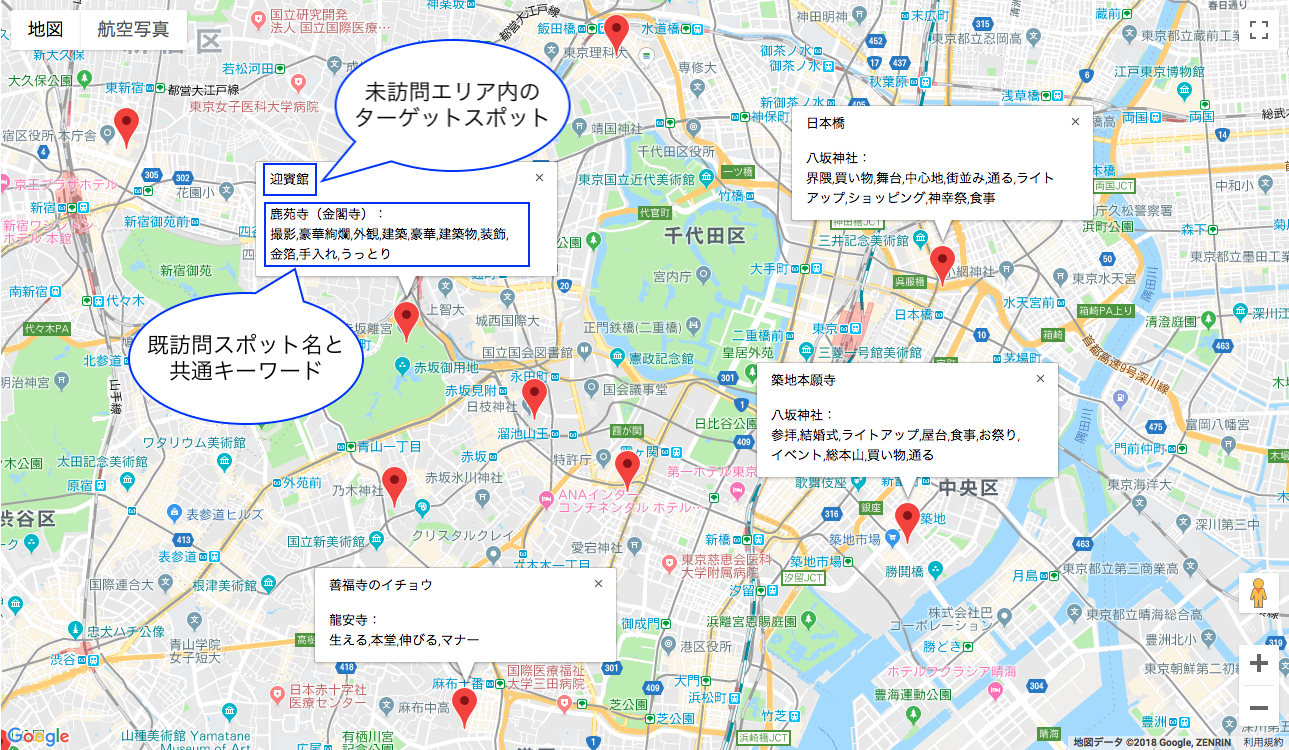
\includegraphics[width=0.9\textwidth]{./figure/map_jap.png}
    \caption{プロトタイプシステム}
    \label{fig:プロトタイプシステム}
   \end{center}
\end{figure}

%%%%%%%%%%%%%%%%%%%
\section{検索結果スポットと既訪問スポットの対応付け}
\label{sec:検索結果スポットと既訪問スポットの対応付け}
検索結果スポットを理解しやすくするために,最も位置付けの近いユーザの既訪問スポットを対応付ける手法を提案する.
まず,ユーザがすでに訪問した複数個の観光スポットとこれから訪問したい観光スポットエリア情報を入力する.
本手法では,観光スポットのユーザレビューを用いて特徴ベクトルを生成する.
この特徴ベクトルには,カテゴリなどのメタデータによるもの,そのスポットのレビュー文から生成した文書ベクトルが一般的である.
さらに本研究では,ユーザの観光地の位置付けを抽出するために,あるスポットに対し他の訪れたスポットと比較した相対的特徴ベクトルを用いる.
同様に,検索結果スポットもエリア内の各スポットの特徴ベクトルを求める.
また,未訪問エリアの各観光スポットの特徴ベクトルを,そのエリアの他の観光スポットと比較して計算する.
次に,特徴ベクトルの類似度によって既訪問スポットを検索結果スポットと対応付ける.
最後に,その関係性を説明するためのキーワードを抽出する.

なお,篠田ら\cite{篠田},藤田ら\cite{藤田}の研究にあるようにGPSなどの位置探知デバイスから自動的にユーザの移動情報を利用して,移動の特徴を分析し興味のあるスポットと取り出す技術もある.
本研究では,ユーザの体験履歴の中でいままで訪れたことがある,かつ気に入った観光スポットを入力することとしているが,このような,位置探知デバイスの技術を使って体験履歴を取得することが可能と考えられる.

%%%%%%%%%%%
\subsection{観光スポットのユーザレビューを用いた特徴ベクトル生成と対応付け}
\label{subsec:観光スポットのユーザレビューを用いた特徴ベクトル生成と対応付け}
本研究では,スポットの特徴ベクトル生成にParagraph Vectorモデルを用いる.
Paragraph Vectorモデルは,Mikolovら\cite{Mikolov}によって考案された単語の特徴ベクトル学習手法であるword2vecを拡張し,Leら\cite{Le}によって提案された文書の特徴ベクトル学習手法である.
Paragraph VectorモデルではHarrisの分布仮説 \cite{Harris}\footnote{Harrisの分布仮説は単語の分散モデルでも使われており,「同じ文脈で出現する単語は類似した意味を持つ」という仮説である.}に基づき,「ある文書中である単語列を与えられたとき,次に出現する単語を予測する」というタスクをニューラルネットワークに学習させることで,文脈や単語の語順を考慮した文書の特徴ベクトルを生成することができる.
Paragraph Vectorモデルでは,生成した文書の特徴ベクトルを文書の分散表現と呼ぶ.

分散表現を用いて観光スポットの特徴ベクトルを作成する.
このとき,観光スポット毎のレビューをまとめて1つの文書として扱う.
本研究では,分散表現を計算するためにPythonのライブラリであるgensim\footnote{https://radimrehurek.com/gensim/models/doc2vec.html}を利用する.
学習方法として,Distributed Bag-of-Wordsを利用して,各スポットの全レビューを使って300次元で作成したベクトルを使う.
既訪問スポットや検索結果スポットのレビューベクトルは,形態素解析器であるMeCab\cite{Kudo}に辞書「mecab-ipadic-NEologd」\footnote{https://github.com/neologd/mecab-ipadic-neologd/}用いて,分かち書きし原形にしたレビューを利用して作成する.
このようにしてできた一般的な文書ベクトルを本論文では,分散表現ベクトルと呼ぶ.

それに対し,本研究における観光スポットの対応付けに関して,ユーザによって,その強調するべき特徴が変化する場合がある.
たとえば,日本の有名な観光スポットを履歴に持つユーザにとっての「金閣寺」の特徴は,お寺,金色,京都などである.
それに対し,京都の寺院を履歴に持つユーザにとっての「金閣寺」の特徴は,金色,金箔,輝きなどとなり.同じ「金閣寺」でもお寺や京都などは特徴にはない.
このような特徴を相対的特徴と定義する.
このような相対的特徴は履歴中の代表的な特徴を打ち消すことで抽出できると考えた.
そこで,あるスポットに対し他の訪れたスポットと比較した相対的特徴ベクトル$r_{state,i}$を,式\ref{math:Vector difference}として定義する.
\begin{equation}
  r_{state,i}=s_i-average(\{	s|s \in S_{state},s \neq s_i \})
  \label{math:Vector difference}
\end{equation}
相対的特徴ベクトルは,そのスポット自体の分散表現ベクトルから他のスポットの分散表現ベクトルの平均を引いた値によって得られる.
$S_{state} =\{s_1,s_2,\dots,s_n\}$は,既訪問スポットもしくは検索結果スポットのベクトル集合である.
$state$が$f$であれば,既訪問スポット集合を意味し,$state$が$u$であれば,検索結果スポット集合を意味する.
$s_i$は集合$S_{state}$内の観光スポット$i$の分散表現ベクトルを示している.

未訪問エリア内のスポットを既訪問スポットと対応付ける.
具体的には,ある検索結果スポットの特徴ベクトルに最も類似度が高い既訪問スポットを対応付ける.
類似度計算には,コサイン尺度を用いる.
ただし,類似度が閾値以下である場合は対応付けを行わない.

% 図\ref{fig:分散表現ベクトルによる対応付けと相対的特徴ベクトルによる対応付け}の左側はスポットの分散表現ベクトルによる対応付けのイメージ図,右側はスポットの相対的特徴ベクトルによる対応付けのイメージ図である.
% 左側は検索結果スポットと既訪問スポットの類似度を計算して,スポット間の特徴で対応付けを行なっている.
% 右側はあるスポットに対し他の訪れたスポットと比較した結果の類似度を計算して,スポットの相対的特徴で対応付けを行なっている.
% \begin{figure}[t]
%   \begin{center}
%     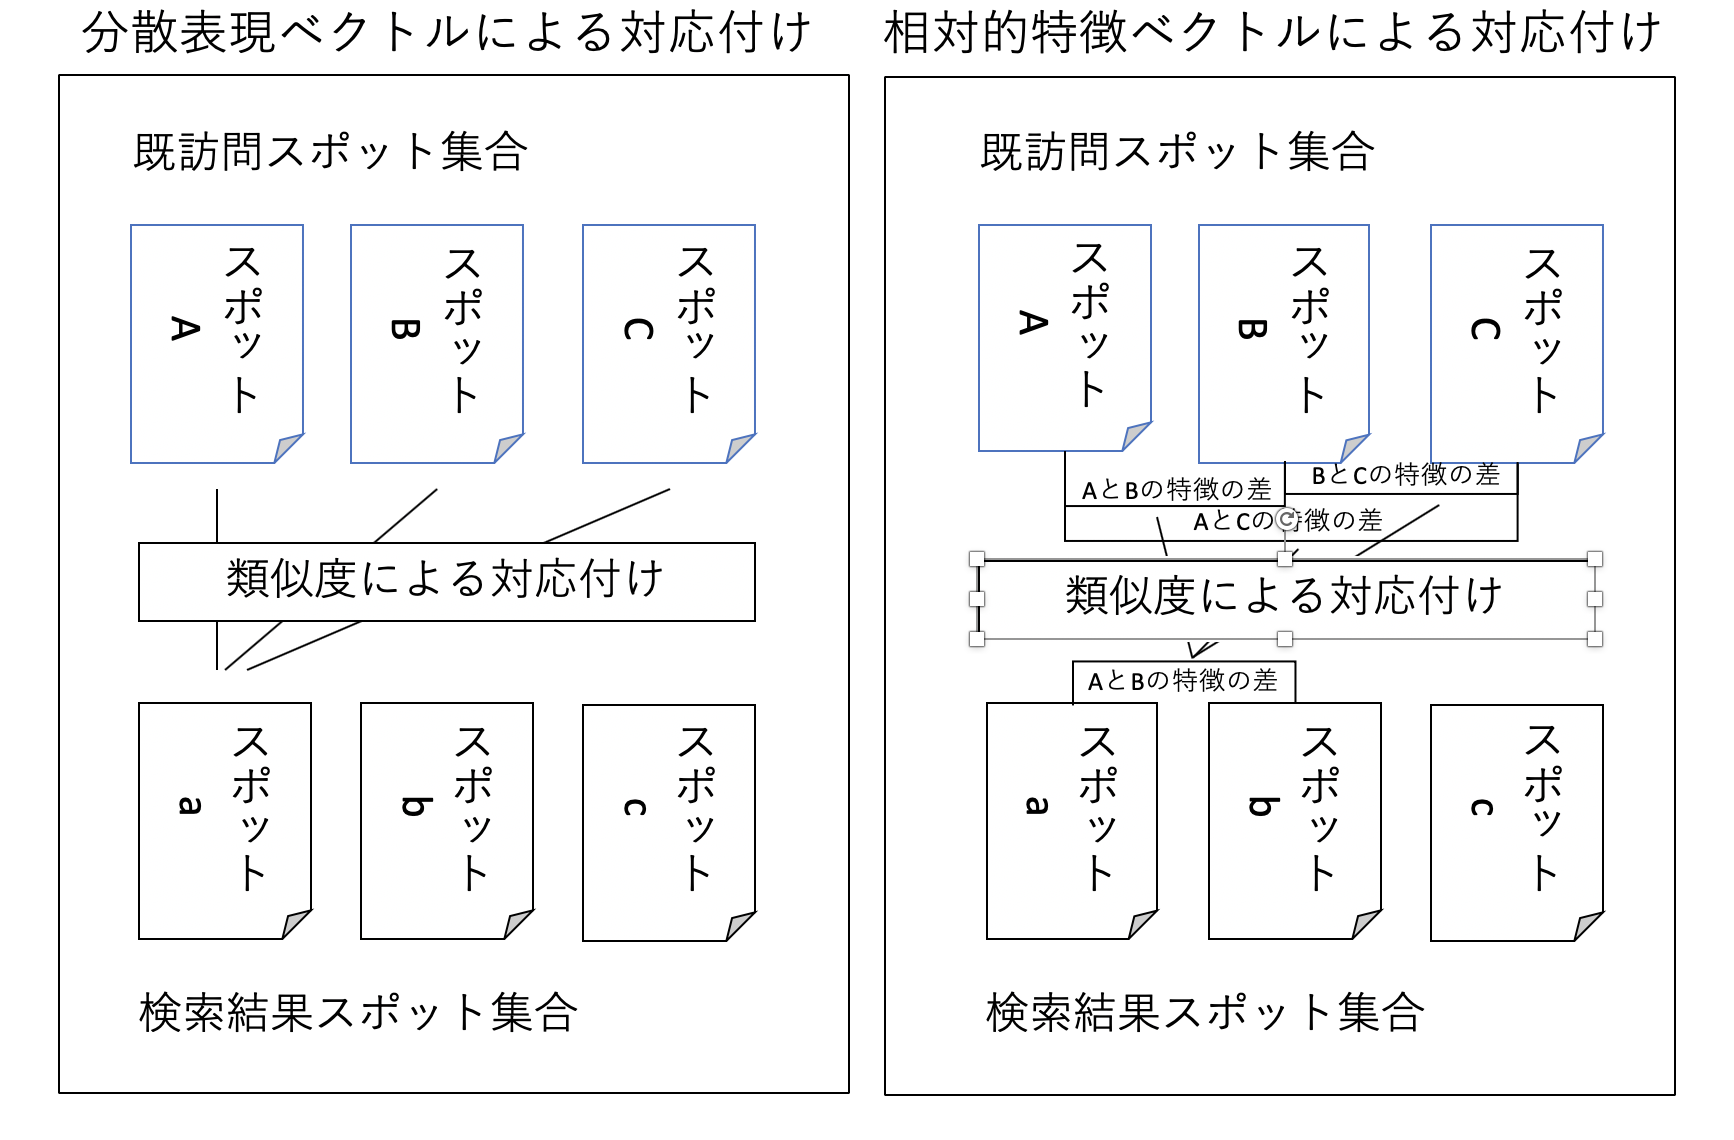
\includegraphics[width=0.9\textwidth]{./figure/better.png}
%     \caption{分散表現ベクトルによる対応付けと相対的特徴ベクトルによる対応付け}
%     \label{fig:分散表現ベクトルによる対応付けと相対的特徴ベクトルによる対応付け}
%   \end{center}
% \end{figure}

カテゴリなどのメタデータによる対応付け手法を説明する.
この対応付けはここまでと異なり,特徴ベクトルではなく,観光スポット検索サイトでスポットを検索するためのメタデータであるカテゴリ,滞在時間,訪問時期の一致を用いる.
まず,検索結果スポットに対し,すべてが一致する既訪問スポットを抽出する.
抽出できない場合は,季節,滞在時間,カテゴリの順に条件を緩和する.
既訪問スポットが複数ある場合は,レビュー数が最も多いスポットを選択する.
メタデータの例を以下に示す.
\begin{itemize}
 \item カテゴリ:神社・神宮・寺院,観光施設・名所巡り等
 \item 滞在時間:1時間未満,1--2時間等
 \item 訪問時期:1--12月,春,夏,秋,冬
\end{itemize}

%%%%%%%%%%%
\subsection{対応する観光スポットの特徴語抽出}
\label{subsec:対応する観光スポットの特徴語抽出}
観光スポットの対応関係を示すだけでは,どのような点で対応するのかを理解するのは難しい.
そこで,検索結果スポットと既訪問スポットの関係性を表すキーワードをユーザに提示する.
しかし,メタデータそのものや,分散表現である特徴ベクトルから単語の特徴を得ることはできないため,他の方法を用いて単語を抽出する.

すべてのレビューを\ref{subsec:観光スポットのユーザレビューを用いた特徴ベクトル生成と対応付け}節と同様に形態素解析器MeCabによって単語に分割する.
ただし,助詞,助動詞,連体詞,記号,ストップワードを削除している.

キーワード抽出手順について説明する.
まず,TF-IDF法を使って対象となる既訪問スポットと検索結果スポットの特徴語とTF-IDF値を求める.
IDF値\cite{IDF}を算出する集合は$S_{state}$を用いる.

2つのスポットに共通する特徴語のTF-IDF値の調和平均を用いて,対応付けしたスポットの説明可能なキーワードとして抽出する.
各単語のスコアを式\ref{math:Harmonic Mean}によって定義する.
\begin{eqnarray}
  score(t,s_f,s_u) = \frac{2 \times tfidf(t,s_f) \times tfidf(t,s_u)}{tfidf(t,s_f) + tfidf(t,s_u)}
  \label{math:Harmonic Mean}
\end{eqnarray}
$tfidf(t,s_f)$と$tfidf(t,s_u)$は同じ単語に関する既訪問スポット$s_f$におけるTF-IDF値と検索結果スポット$s_u$におけるTF-IDF値を示している.
単語スコアの上位$N$個の単語を説明情報としてユーザに提示する.

%%%%%%%%%%%
\subsection{実行例}
\begin{table}[t]
  \caption{既訪問スポット集合と検索結果スポット集合}
  \label{table:既訪問スポット集合と検索結果スポット集合}
  \centering
  \begin{tabular}{l|l}
  \hline
  \multicolumn{1}{c|}{既訪問スポット名} & \multicolumn{1}{c}{検索結果スポット名} \\ \hline
  浅草寺                           & 東京ディズニーランド(R)                \\
  小田原城址公園                       & 新宿御苑                         \\
  伏見稲荷大社                        & 東京スカイツリー                     \\
  奈良公園                          & 東京タワー大展望台                    \\
  三島スカイウォーク                     & 明治神宮                         \\ \hline
  \end{tabular}
\end{table}

\begin{table*}[t]
    \caption{対応付け結果の例}
    \label{table:対応付け結果の例}
    \centering
    \begin{tabular}{l|l|l}
    \hline
    \multicolumn{1}{c|}{検索結果スポット} & \multicolumn{1}{c|}{既訪問スポット} & \multicolumn{1}{c}{特徴語}                                                                \\ \hline
    新宿御苑                         & 小田原城址公園                      & \begin{tabular}[c]{@{}l@{}}お花見,咲き誇る,園内,桜の時,のんびり,\\ 手入れ,自然,遊具,ツツジ\end{tabular}          \\ \hline
    東京スカイツリー                     & 三島スカイウォーク                    & \begin{tabular}[c]{@{}l@{}}富士山,揺れ,高所恐怖症,揺れる,天井,絶景,\\ エレベーター,パノラマ,展望デッキ,昇る\end{tabular} \\ \hline
    \end{tabular}
\end{table*}

表\ref{table:既訪問スポット集合と検索結果スポット集合}に示す,既訪問スポット集合と検索結果スポット集合を用いて相対的特徴ベクトルを用いて対応付けを行った結果を説明する.
検索結果スポットは首都圏内を想定し5つのスポットを選んだ.
表\ref{table:対応付け結果の例}は,\ref{sec:検索結果スポットと既訪問スポットの対応付け}節で述べた提案手法を用いて抽出した対応付いたスポットの特徴語を示している.

検索結果スポット「新宿御苑」に対し,既訪問スポット「小田原城址公園」が対応付いた.
他の候補として「奈良公園」が考えられるが,「小田原城址公園」には花や遊具に対する記述が多く,「奈良公園」には鹿や草に対する記述が多い.
「新宿御苑」には花や遊具に対する記述が多いため,「小田原城址公園」と適切に対応付けたと考える.

検索結果スポット「東京スカイツリー」に対し「三島スカイウォーク」が対応づけられた.
どちらも眺めや高さに特徴があり関連付けられたと考えられる.
また,特徴語を見ると「富士山」が抽出されており,見える景色を想起させるような対応付けを行っていると考える.

%%%%%%%%%%%%%%%%%%%
\section{対応関係を表す特徴語抽出の評価}
\label{sub:対応関係を表す特徴語抽出の評価}
%%%%%%%%%%%
\subsection{実験内容}
本実験では,2016年9月末までのじゃらん\footnote{https://www.jalan.net/kankou/}から得られたレビューデータを用いる.
また,本実験において類似度を計算するときの閾値を0.125とする.
これは,以降の\ref{sub:観光スポットの対応付けに関する評価}節,\ref{sub:検索結果スポット説明の有効性評}節の実験でも同様である.
提案手法のうちの特徴語抽出部分について評価を行うため,他のキーワード抽出手法と比較して評価を行う.
なお,特徴ベクトルは相対的特徴ベクトルに固定している.
以下の3つの方法を比較する.
\begin{itemize}
  \item 算術平均法
  \item 乗算法
  \item 調和平均法
\end{itemize}

\begin{table}[t]
  \caption{対応関係を表す特徴語の実験結果}
  \label{table:対応関係を表す特徴語の実験結果}
  \centering
  \begin{tabular}{c|c|c|r|r|r}
  \hline
  選択肢 & \multicolumn{1}{c|}{スポット関係} & \multicolumn{1}{c|}{キーワード} & \multicolumn{1}{c|}{算術平均法} & \multicolumn{1}{c|}{乗算法} & \multicolumn{1}{c}{調和平均法} \\ \hline
  1  & あり & 明確になった & 28.28\%                  & 31.31\%                  & 29.29\%                 \\
  2  & あり & 初めて気づいた & 35.35\%                  & 31.31\%                  & 35.35\%                 \\
  3  & あり & ない & 10.10\%                   & 14.14\%                  & 12.12\%                 \\
  4  & ない & ー & 26.26\%                  & 23.23\%                  & 23.23\%                 \\ \hline
  \end{tabular}
\end{table}

キーワードを抽出するとき,算術平均法では,2つのスポットに共通する特徴語のスコアとして算術平均を計算する.
抽出した単語のスコアを式\ref{math:Mean}によって定義する.
\begin{eqnarray}
  score(t,s_f,s_u) = \frac{tfidf(t,s_f) + tfidf(t,s_u)}{2}
  \label{math:Mean}
\end{eqnarray}

乗算法では,2つのスポットに共通する特徴語のスコアとして乗算を計算する.
抽出した単語のスコアを式\ref{math:Multi}によって定義する.
\begin{eqnarray}
  score(t,s_f,s_u) = tfidf(t,s_f) \times tfidf(t,s_u)
  \label{math:Multi}
\end{eqnarray}

%%%%%%%%%%%
\subsection{実験手順}
\label{subsec:実験手順}
クラウドソーシングのサービスである,CrowdWorks\footnote{https://crowdworks.jp/}を利用して23人の被験者を集めた.
まず,被験者は4個から10個の自分がすでに訪れたことのある観光スポットを入力した.
次に,被験者は旅行などで行ったことがなく,これから訪れたい都道府県やエリアを入力した.

本実験では,それぞれの手法において,対応付けられた既訪問スポットと検索結果スポット,およびスポット同士の関係を説明する特徴語を最大で5つまで提示した.
結果を評価するために,被験者は以下の4つの選択肢から1つを選んだ.
\begin{enumerate}
  \item 2つのスポットには関係性があり,キーワード\footnote{関係を説明する特徴語のことであるが,被験者には単にキーワードと示した.}によって関係が明確になった.
  \item 2つのスポットの関係性があり,キーワードによって初めて気がついた.
  \item 2つのスポットには関係性があるが,キーワードは関係を表していない.
  \item 2つのスポットには関係性がない.
\end{enumerate}

%%%%%%%%%%%
\subsection{実験結果と考察}
表\ref{table:対応関係を表す特徴語の実験結果}は,それぞれの手法における選択肢1から4それぞれの選択割合を示している.
乗算法では,多くの被験者が選択肢1を選択している.
このことから,乗算法は明らかな関係を表現する特徴語抽出ができることがわかった.
算術平均法と調和平均法では,選択肢1の割合が減少し,選択肢2の割合が増加している.
このことから,算術平均法と調和平均法は隠れた関係を表現する特徴語を見つけて被験者に提示することができると考えた.

しかし,算術平均法では,選択肢4の割合が増加しているため,調和平均法より無関係な特徴語を抽出しやすくなったといえる.
また,選択肢1と2を合計すると,調和平均法が最も高くなった.
このことから,スポットの関連を説明する特徴語抽出手法としては調和平均法が妥当といえる.

%%%%%%%%%%%%%%%%%%%
\section{観光スポットの対応付けに関する評価}
\label{sub:観光スポットの対応付けに関する評価}
%%%%%%%%%%%
\subsection{実験内容}
特徴語抽出については\ref{subsec:対応する観光スポットの特徴語抽出}節の手法を用いる.
提案手法のうちの対応付け部分について,\ref{subsec:観光スポットのユーザレビューを用いた特徴ベクトル生成と対応付け}節で説明した以下の3つの手法を比較して評価を行う.
\begin{itemize}
  \item メタデータ法
  \item 分散表現法
  \item 相対的特徴法
\end{itemize}

クラウドソーシングのサービスである,CrowdWorksを利用して24人の被験者を集めた.
実験手順は\ref{subsec:実験手順}節で説明した手順と同様である.

%%%%%%%%%%%
\subsection{実験結果と考察}
\begin{table}[t]
  \caption{対応付けに関する実験結果}
  \label{table:対応付けに関する実験結果}
  \centering
  \begin{tabular}{c|c|c|r|r|r}
  \hline
  選択肢 & \multicolumn{1}{c|}{スポット関係} & \multicolumn{1}{c|}{キーワード} & \multicolumn{1}{c|}{メタデータ法} & \multicolumn{1}{c|}{分散表現法} & \multicolumn{1}{c}{相対的特徴法} \\ \hline
  1  & あり & 明確になった & 41.30\%                    & 33.85\%                    & 29.36\% \\
  2  & あり & 初めて気づいた & 43.48\%                    & 47.69\%                    & 48.62\% \\
  3  & あり & 関係なし & 2.17\%                     & 2.31\%                     & 2.75\% \\
  4  & ない & ー & 13.04\%                    & 16.15\%                    & 19.27\% \\
  \hline
  対応付け数  &&& 46                    & 130                    & 109 \\
   \hline
  \end{tabular}
\end{table}

対応付けしたスポットの合計数は285である.
表\ref{table:対応付けに関する実験結果}は,それぞれの方法における選択肢1から5それぞれの選択割合を示している.
メタデータ法について,多くの被験者が選択肢2を選択している.
このことから,メタデータ法は明らかな関係にあるスポット同士を関連付けることができることがわかった.
他の方法と比較して,相対的特徴法では,選択肢1の割合が減少し,選択肢2の割合が増加している.
このことから,相対的特徴法は隠れた関係を見つけて被験者に提示することができると考えた.
しかし,選択肢4の割合も増加しているため,無関係なスポットを抽出しやすくなったといえる.

選択肢1と2を合計すると,メタデータ法が最も高くなる.
このことから,説明するためのスポットの対応付けの精度が最も高いといえる.
しかし,メタデータ法は対応付けすることができるスポットの数が他の手法に比べ半分以下であり,多くの検索結果スポットに説明を付与することができない.

分散表現法と相対的特徴法を詳細に考察するために,既訪問スポットの入力別に比較した.
入力した既訪問スポットの半数以上が同一カテゴリのスポットであった被験者(表中の「同じ場合」)とそうではない被験者(表中の「異なる場合」)に分けて集計した.
表\ref{table:既訪問スポットのカテゴリの同異による評価割合}は選択肢1と選択肢2の評価の割合である.
相対的特徴法を使用すると,カテゴリが異なる場合において,分散表現法よりも選択肢1および選択肢2の割合を増加させることができる.
相対的特徴ベクトルを用いることによって,カテゴリをこえて各スポットの特徴を求めることができるといえる.
カテゴリが同じ場合の選択肢1は相対的特徴法では,少なくなっている.
これは,相対的特徴ベクトルとしては,カテゴリの特徴が打ち消されたベクトルが生成されるため,明らかな関係となる対応付けが減ったと考えられる.
しかし,選択肢2が増えずに選択肢4が増え,無関係に見える対応付けを増やす結果となった.
そのため,入力スポットの種類によって対応付け手法を切り変えることが有効と考えられる.

\begin{table}[t]
  \caption{既訪問スポットのカテゴリの同異による評価割合}
  \label{table:既訪問スポットのカテゴリの同異による評価割合}
  \centering
  \begin{tabular}{c|c|r|r}
  \hline
  & 選択肢 & \multicolumn{1}{c|}{分散表現法} & \multicolumn{1}{c}{相対的特徴法} \\ \hline
  異なる場合                 & 1   & 19.23\%                  & 21.10\%                 \\ \cline{2-4}
  & 2   & 24.62\%                  & 25.69\%                 \\ \hline
  同じ場合                  & 1   & 14.62\%                  & 8.26\%                  \\ \cline{2-4}
  \multicolumn{1}{l|}{} & 2   & 23.08\%                  & 22.94\%                 \\ \hline
  \end{tabular}
\end{table}


%%%%%%%%%%%%%%%%%%%
\section{検索結果スポット説明の有効性評価}
\label{sub:検索結果スポット説明の有効性評}
%%%%%%%%%%%
\subsection{実験内容}
提案手法の有効性を評価するために以下の2つのシステムを使って比較する.
提案手法では,対応付けに相対的特徴法,キーワード抽出に調和平均法を用いた.
\begin{description}
  \item a.検索結果スポット名のみを表示
  \item b.検索結果スポット名,対応する入力スポット,対応を説明する特徴語を表示(提案手法)
\end{description}

被験者の入力は,これまでの実験と同様に,4個から10個の自分がすでに訪れたことのある観光スポットと訪問したいエリアである.
ただし,エリアは2つ入力し,それぞれ別々にシステムa,システムbの入力として用いた.
なお,システムaとシステムbはランダムな順番で実行される.
システムを評価するために,被験者は以下の2つの設問について回答した.
また,それらの選択理由について自由記述で答えた.
\begin{description}
  \item Q1. 表示されたスポットの詳細情報はどちらの方が分かりやすいかを選択してください.
  \item Q2. 旅行の計画を立てる際にどちらの方が使いたいかを選択してください.
\end{description}

被験者はクラウドソーシングのサービスである,CrowdWorksを利用して集めた50人を用いた.

%%%%%%%%%%%
\subsection{実験結果と考察}
Q1に対する回答について,システムaとシステムbの結果はそれぞれ12件と38件となった.
被験者の回答理由の例を表\ref{table:システムaの方が良いと回答した被験者の自由記述}(システムa)および,表\ref{table:システムbの方が良いと回答した被験者の自由記述}(システムb)に示す.
また,
旅行の計画を立てる際にどちらの方が使いたいかに対する回答について,システムaとシステムbの結果はそれぞれ10件と40件となった.
被験者の回答より,得られた2つのシステムの特徴をまとめる.

システムbでは,キーワードや関連している情報が表示されており分かりやすいという特徴がある.
これに対し,システムaでは,スポット名のみが表示されているためシンプルで分かりやすいという特徴があるが,「なぜそのスポットが検索されたのか分からない」などの否定的な回答も多数あった.
システムの表示情報が「シンプルな方が良い」と「詳細な情報が良い」の2つに大きく分けられているが,Q2の回答より80\%の被験者はシステムbの方が使いたいと回答しており,提案手法の方の評価が高いといえる.
また,システムbに関してスポットの写真を載せるとより分かりやすいなどの意見があり,画像による関連性の説明という拡張が考えられる.

\begin{table}[t]
  \caption{システムaの方が良いと回答した被験者の自由記述}
  \label{table:システムaの方が良いと回答した被験者の自由記述}
  \centering
  \begin{tabular}{l}
  \hline
  \begin{tabular}[c]{@{}l@{}}スポット名だけ書いてあるのでごちゃごちゃにならず、一目でどこに\\ 何があるか分かるからです.\end{tabular} \\ \hline
  スポットだけ表示されるところがシンプルで分かりやすかったから.                                                         \\ \hline
  シンプルにそのエリアの観光スポットを知ることが出来る.                                                             \\ \hline
  \end{tabular}
\end{table}

\begin{table}[t]
  \caption{システムbの方が良いと回答した被験者の自由記述}
  \label{table:システムbの方が良いと回答した被験者の自由記述}
  \centering
  \begin{tabular}{l}
  \hline
  自分が訪れた事のあるスポットと関連性があり連想しやすいから.                                                 \\ \hline
  \begin{tabular}[c]{@{}l@{}}どのような場所か想像しやすいので、計画を立てるのにも使いたい\\ と思ったから.\end{tabular} \\ \hline
  何と関連して表示された等詳細の情報が表示されわかりやすかった.                                                  \\ \hline
  \end{tabular}
\end{table}

%%%%%%%%%%%%%%%%%%%
\section{まとめ}
観光スポットを効果的に理解するために,観光スポット間の対応付けを行い,検索結果スポット説明の有効性を評価する実験を行った.
検索結果スポットを簡単に理解するためには,ユーザにどのような情報を提示することによって理解につながるかが重要である.
従来では,カテゴリ,滞在時間などのメタデータを使って観光スポットの検索を行い,そのあと検索したあとに,検索結果スポットをひとつずつ見ていくことが多くなっている.
これでは,ユーザにとって理解するための時間と労力が必要となり,検索結果スポットを効果的に理解することにつがらない.
検索結果スポットを効果的に理解するために,ユーザがいままで訪問したことのある既訪問スポットを用いて検索結果スポットを説明することが効果的であると考えられる.
また,検索結果スポットを説明するためにその特徴語を表示することが効果的と考えられる.
対応付けよる説明を効果的にするために,既訪問スポットと検索結果スポットの対応付けは,レビューを用いて作成した相対的特徴ベクトルによる類似により詳細な対応付けを行う.

\ref{sub:対応関係を表す特徴語抽出の評価}節では,相対的特徴ベクトルで対応付けした既訪問スポットと検索結果スポットの特徴語抽出方法の評価実験を行った.
その結果,調和平均の計算による単語抽出の方が妥当であることを明らかにした.

\ref{sub:観光スポットの対応付けに関する評価}節では,メタデータ法,分散表現法,相対的特徴法の3つの手法で対応付けの実験を行った.
ユーザに提示する情報は\ref{sub:対応関係を表す特徴語抽出の評価}節で確認した調和平均によって抽出した特徴語である.

メタデータでは,高速に観光スポットの検索ができるが,絞り込みによって検索される結果が少なくなる.
メタデータに対して,分散表現と提案手法では対応付けするために処理する時間がかかる.
また,メタデータによる検索結果スポットはユーザが設定した大きな利用目的から逸脱することはなく,ユーザがこれから訪問したい特定のカテゴリに収まることが多いため,利用目的が明確な場合においてメタデータ法はユーザにとって理解しやすい.

提案手法において,相対的特徴ベクトルを利用した場合,カテゴリの特徴が打ち消されたベクトルが生成され,検索結果スポットはユーザが設定したカテゴリ情報だけでなく,より詳細な特徴を持つ検索結果スポットの特徴語が提示される.
提案手法によって提示した検索結果スポットの特徴語は,ユーザにとって新しい説明情報としてスポットの理解につながる.

観光スポットを効果的に理解する点において,ユーザはこれから訪問したいエリアに対して,カテゴリがすでに決まっている場合では,メタデータ法で検索された観光スポットが効果的に理解しやすいと考えられる.
それに対し,ユーザは訪問したいエリアのスポットに対してより詳細な情報を知りたい場合,相対的特徴ベクトルで対応付けしたスポット間の特徴語を提示することによって効果的に理解しやすいと考えられる.

観光スポットを効果的に理解するために,ユーザに検索結果スポット名だけではなく,対応する既訪問スポットとそれを説明する特徴語を加えることが理解につながると考えられる.
地図上では一般的な検索結果はスポット名や場所情報がユーザに表示されるが,\ref{sub:検索結果スポット説明の有効性評}節では,対応する既訪問スポットと説明するための特徴語を提示することによる説明の有効性評価を行った.
特徴語と対応する既訪問スポットを提示することによって,検索結果スポットとの関連性が連想しやすくなり,観光スポットを効果的に理解することにつながる.

\ref{sub:対応関係を表す特徴語抽出の評価}節,\ref{sub:観光スポットの対応付けに関する評価}節,\ref{sub:検索結果スポット説明の有効性評}節で行った3つの評価実験を通し,相対的特徴ベクトルを利用して,対応付けした方がより観光スポットの詳細を理解することができると考えられる.

%%%%%%%%%%%%%%%%%%%%%%%%%%%%%%%%%%%%%%%%%%
\chapter{地図上における検索結果スポットの説明性向上のための観光スポットの対応関係可視化手法}
\label{cha:地図上における検索結果スポットの説明性向上のための観光スポットの対応関係可視化手法}
%%%%%%%%%%%%%%%%%%%%%%%%%%%%%%%%%%%%%%%%%%
本章では,観光スポット間の対応関係を地図上に可視化する手法を提案する.
また,プロトタイプシステムを構築し,既訪問スポットと検索結果スポットの説明性向上のための観光スポットの対応関係を地図上に可視化した効果を評価する実験を行う.

%%%%%%%%%%%%%%%%%%%
\section{概要}
近年,ユーザはWeb上の観光情報を活用して旅行計画を立てることが多くなっている.
しかし,旅行は一般的に訪れたことがないスポットに行くことが多いため,観光情報を適切に理解することは困難である.
そこで,訪問したことがある観光スポットの特徴を用いて,未訪問エリアの観光スポットを対応付けを行い,ユーザの未知なスポットに対する理解を支援する.
観光スポット間の対応関係を地図上に可視化する手法を提案する.

本手法では,まず,3章で述べた手法により,スポットの特徴ベクトル間の類似度に基づいて既訪問スポットと検索結果スポットを対応付けし,その対応関係を説明するための特徴語を抽出する.
次に,地図上で表示するための意味的な位置関係を決定する.
具体的には,検索結果スポットからの地理的な距離と類似度によって存在度を決定して,意味的な位置関係に基づいて観光スポットの対応関係をわかりやすくするための既訪問スポットの座標を算出する.
また,プロトタイプシステムを構築し,既訪問スポットと検索結果スポットの説明性向上のための観光スポットの対応関係を地図上に可視化した効果を評価する実験を行う.

%%%%%%%%%%%%%%%%%%%
\section{観光スポット間の対応関係を用いた可視化}
検索結果スポットを理解しやすくするために,もっとも位置付けの近いユーザの既訪問スポットを対応付ける手法を提案した.
この手法では,3章で述べた対応付けを前提としている.
ユーザがすでに訪問した複数個の観光スポットとこれから訪問したい観光エリアを入力とする.
ユーザが入力した観光スポット集合のユーザレビューを用いてそれぞれのスポットの特徴ベクトルを生成する.
同様に,検索結果スポットもエリア内の各スポットの特徴ベクトルを求める.
次に,特徴ベクトルのコサイン類似度によって既訪問スポットを検索結果スポットと対応付ける.
最後に,その関係性を説明するためのキーワードをTF-IDF特徴量と調和平均で抽出する.

ある検索結果スポットに対して,入力した既訪問スポットがどのような関係にあるのか地図上で,一目で把握できることが望ましい.
ユーザは地図上で観光スポットを検索しているものとし,まず,地図上の実際にスポットが存在する座標に検索結果スポットを配置する.
次に,既訪問スポットの位置を決定する.
これは検索結果スポットとの対応関係によって変化し,検索結果スポットとの類似度が高いと近く,類似度が低いと遠くなるように配置することで,意味的な位置関係を表現する.
既訪問スポットの座標は,式\ref{math:score}によって求める.
\begin{eqnarray}
Score(s_f,T) = \sum_{s_u \in S_u}^{} w(s_u,s_f) \times P_{s_u,s_f}(d(s_u,T))
    \label{math:score}
\end{eqnarray}
$S_u$を未訪問エリア内のスポット集合とする.
$w(s_u,s_f)$は,ある既訪問スポット$s_f$と検索結果スポット$s_u$の類似度が正であれば$1.0$,負であれば$-0.5$を返す関数である.
$T$は,候補の座標である.
$d(s_u,T)$は,ある座標$T$から検索結果スポット$s_u$のユークリッド距離である.
また,$P_{s_u,s_f}$は,平均$\mu$が$0$,標準偏差$\sigma$が$(1-|cos(vec(s_u),vec(s_f))|) \times \alpha$である正規分布を表す.
$\alpha$は重みである.
$vec$は検索結果スポットや既訪問スポットの特徴ベクトルを返す関数である.
$Score(s_f,T)$がもっとも大きな座標$T$を既訪問スポットの座標とする.

図\ref{fig:image}は既訪問スポットの経度座標計算の例である.
縦軸はスコアの値であり,横軸は経度である.
4つの検索結果スポットを用いて,$Score(s_f,T)$(合計スコア)を計算している.
その結果,$135.06$の座標がもっとも高くなる.
緯度についても同様に行う.

\begin{figure}[t]
  \begin{center}
    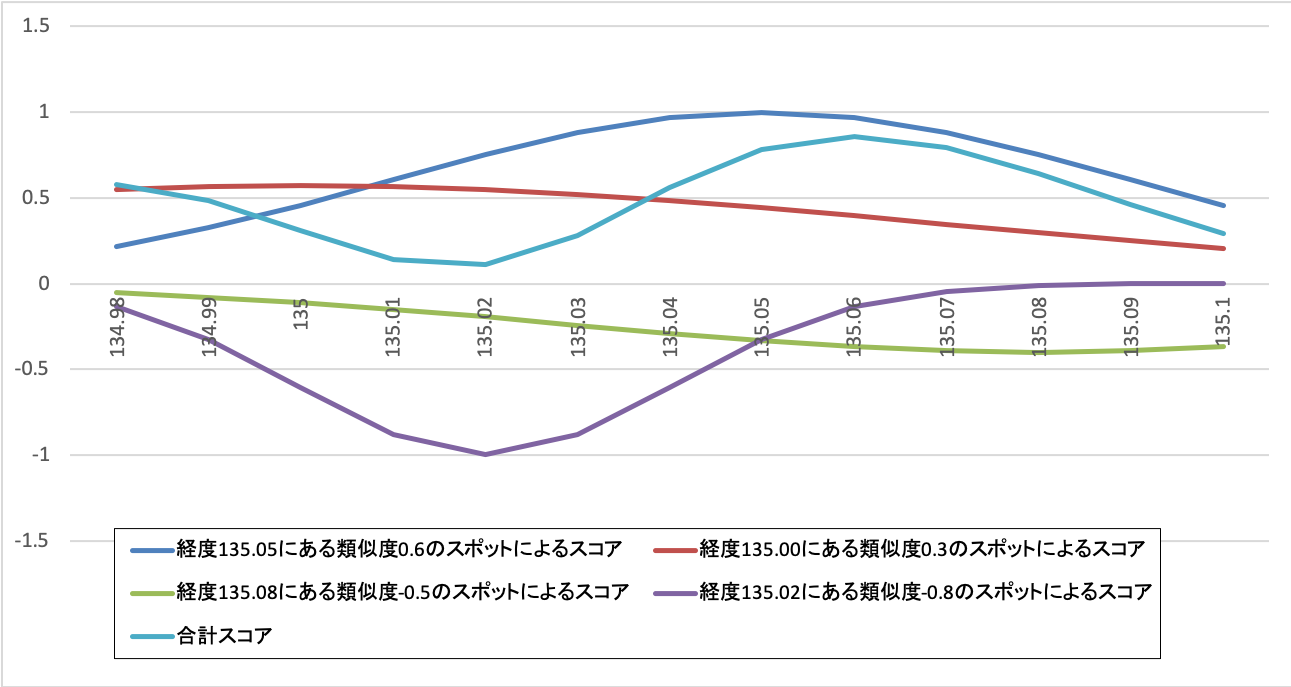
\includegraphics[width=0.9\textwidth]{./figure/score_image.png}
    \caption{既訪問スポットの経度座標計算の例}
    \label{fig:image}
   \end{center}
\end{figure}

%%%%%%%%%%%%%%%%%%%
\section{対応関係の可視化評価}
\label{sec:対応関係の可視化評価}
%%%%%%%%%%%
\subsection{実験内容}
\label{sec:特徴ベクトル実験内容}
検索結果スポットの説明性向上のための観光スポットの対応関係可視化手法の評価を行うため,以下の3つの提示手法を使って比較する.
図\ref{fig:P},図\ref{fig:L},図\ref{fig:T}は3つの提示手法それぞれのプロトタイプシステムとなっている.
黒いマーカーは入力した既訪問スポット,赤いマーカーは未訪問エリア内のスポットを意味している.
表示が重なることもあるため,黒いマーカーをクリックすると既訪問スポット名を吹き出しでも表示する.
また,3つの提示手法において,類似度が類似度の平均以下であれば,関係を表現するキーワードが「なし」と表示する.
これは意味が小さい関係を表すキーワードは一般的に理解しにくいためである.
\begin{figure*}[t]
	\centering
	\begin{minipage}{.45\textwidth}
		\centering
		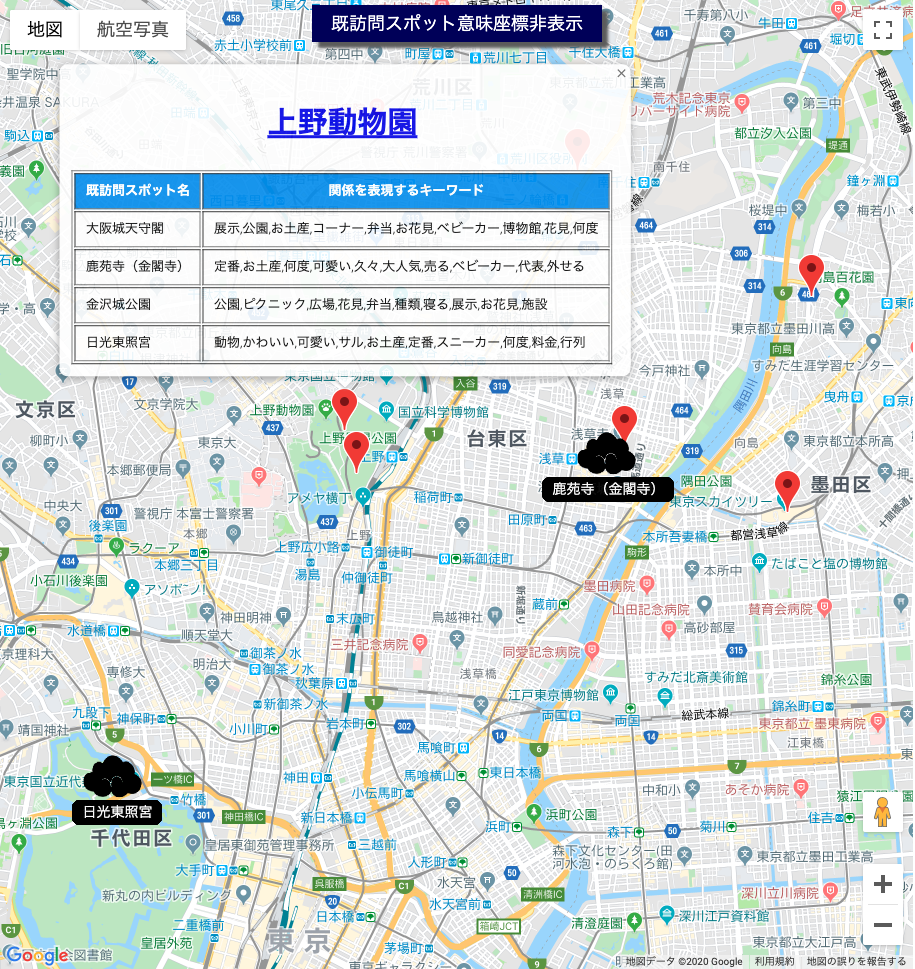
\includegraphics[clip, width=7cm]{./figure/map_p.png}
		\caption{位置関係($Position\_Map$)}
		\label{fig:P}
	\end{minipage}
	%
	\hfil
	%
	\begin{minipage}{.45\textwidth}
		\centering
		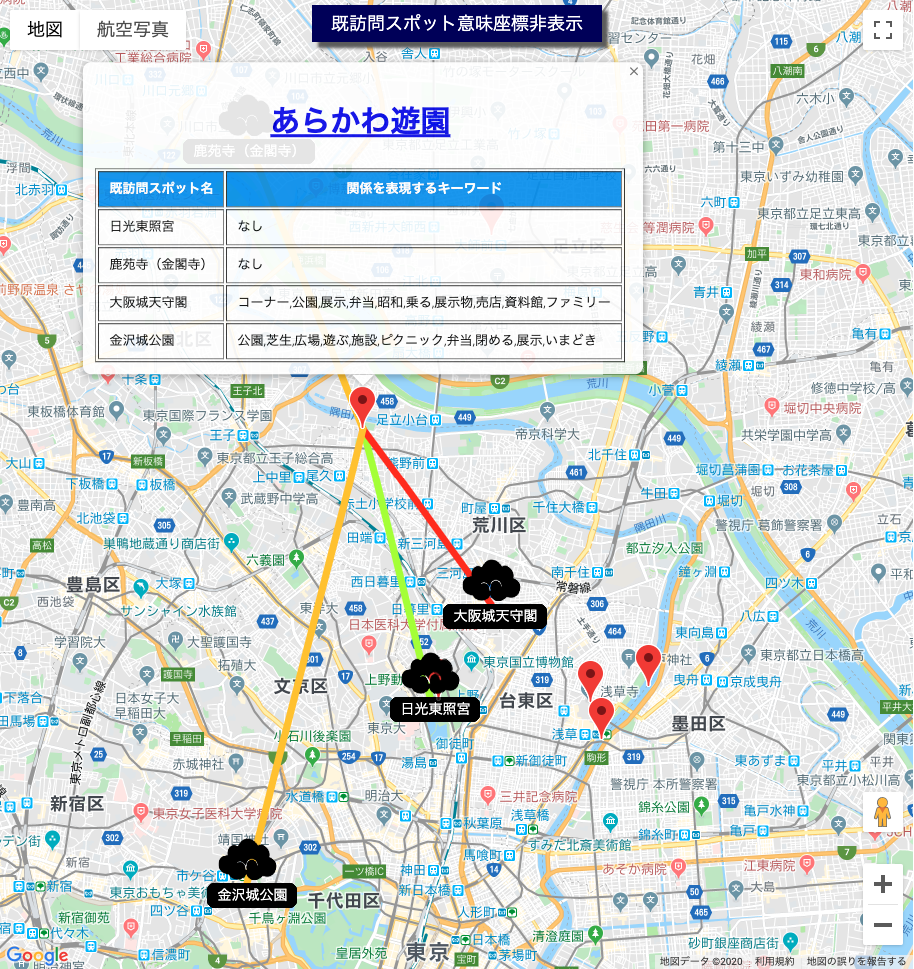
\includegraphics[clip, width=7cm]{./figure/map_l.png}
		\caption{位置関係+線($Line\_Map$)}
		\label{fig:L}
	\end{minipage}
	\hfil
	%
	\begin{minipage}{.45\textwidth}
		\centering
		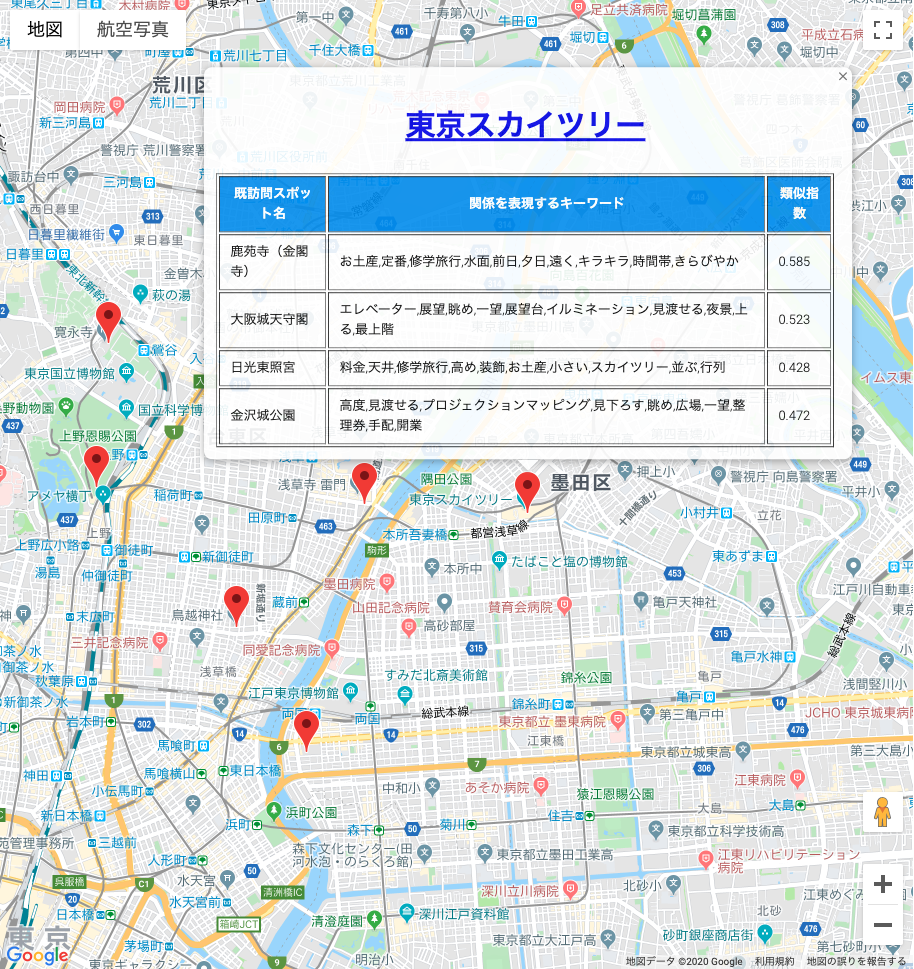
\includegraphics[clip, width=7cm]{./figure/map_t.png}
		\caption{表形式($Table\_Map$)}
		\label{fig:T}
	\end{minipage}
\end{figure*}

$Position\_Map$(図\ref{fig:P})では,検索対象のスポットと既訪問スポットの関連度を全体的な位置関係で表現している.
既訪問スポットは実際の座標ではなく,提案手法で決定した座標で表示される.
赤いマーカーをクリックすると詳細情報が表示される.
詳細情報は,検索結果スポット名,対応する既訪問スポット名,検索結果スポットと既訪問スポットの関係を表現するキーワードである.
「既訪問スポット意味座標(表示/非表示)」ボタンは黒いマーカーの表示/非表示を切り替えることができる.

$Line\_Map$(図\ref{fig:L})では,位置関係による提示に加えて線の色を使って表現している.
線の色は赤いマーカーと黒いマーカーの類似度を示している.
線は緑色に近いと類似度が低く,赤色に近いと類似度が高いことを意味している.
赤いマーカーをクリックすると詳細情報が表示される.
詳細情報は,$Position\_Map$と同じく,検索結果スポット名,対応する既訪問スポット名,検索結果スポットと既訪問スポットの関係を表現するキーワードである.
「既訪問スポット意味座標(表示/非表示)」ボタンは黒いマーカーの表示/非表示を切り替えることができる.

$Table\_Map$(図\ref{fig:T})では,位置関係や線は用いずに,$Line\_Map$で表現していたすべての情報を表形式でまとめて表現している.
詳細情報は,現在選択している検索結果スポット名と,対応する既訪問スポット名,検索結果スポットと既訪問スポットの関係を表現するキーワード,類似度である.
類似度の値は「-1.0から1.0」の間になる.
「-1.0」はもっとも類似せず,「1.0」はもっとも類似することを意味している.

本実験では,近似として対象エリア内を緯度,経度それぞれ17個に分割し,等間隔で代表点を289個作り,それを既訪問スポットの候補点$T$として用いた.
対応関係の可視化を評価するために,観光スポットの相対的特徴ベクトルによる対応関係と分散表現ベクトルによる対応関係の2つの手法を使って比較を行う.
また,本実験においても,特徴ベクトルの生成には,2016年9月末までのじゃらん\footnote{https://www.jalan.net/kankou/}から得られたレビューデータを用いる.

%%%%%%%%%%%
\subsection{実験手順}
クラウドソーシングのサービスである,CrowdWorksを利用して被験者を集めた.
分散表現ベクトルを用いたシステムでは,42人合計60件のデータを集めた.
相対的特徴ベクトルを用いたシステムでは,44人合計60件のデータを集めた.
まず,被験者は3個から9個の自分がすでに訪れたことのある,かつ気に入った観光スポットを入力した.
次に,被験者は旅行などで行ったことがなく,これから訪れたい都道府県やエリアを入力した.

本実験では,各提示手法において,検索スポットが重複しないように振り分け,3つの提示手法を連続して利用した.
それぞれの提示手法において,被験者は検索スポットから行き先を決定した.
このとき,表示順に影響をなくすために,6パターンの表示順を作成し,被験者はランダムに1つの表示順で実験を行う.
実験を行った後,以下の項目について評価する.
\begin{itemize}
  \item 各提示手法の行き先の決定しやすさ
  \item $Position\_Map$と$Line\_Map$どちらの方が,訪問履歴との関係がわかりやすかったか
  \item $Line\_Map$と$Table\_Map$どちらの方が,訪問履歴との関係がわかりやすかったか
  \item 各提示手法の訪問先決定までにかかった体感時間
  \item 各提示手法の訪問先決定までにかかった労力
\end{itemize}
また,それぞれの手法について,自由記述で意見を書いてもらった.

%%%%%%%%%%%
\subsection{分散表現ベクトルを用いた結果と考察}
\begin{table}[t]
    \caption{行き先の決定しやすさの回答数割合(分散表現ベクトル)}
    \label{table:行き先の決定しやすさ(特徴ベクトル)}
    \centering
    \begin{tabular}{l|rrrrr|l}
    \hline
    決定しやすさ   & \multicolumn{1}{l}{1} & \multicolumn{1}{l}{2} & \multicolumn{1}{l}{3} & \multicolumn{1}{l}{4} & \multicolumn{1}{l|}{5} & 平均    \\ \hline
    $Position\_Map$ & 0.0\%                & 18.3\%               & 11.7\%               & 60.0\%               & 10.0\%                & 3.62 \\
    $Line\_Map$     & 1.7\%                & 25.0\%               & 11.7\%               & 43.3\%               & 18.3\%                & 3.52 \\
    $Table\_Map$    & 0.0\%                & 20.0\%                & 23.3\%               & 40.0\%               & 16.7\%                 & 3.53 \\ \hline
    \end{tabular}
\end{table}
表\ref{table:行き先の決定しやすさ(特徴ベクトル)}は3つの提示手法それぞれの行き先の決定しやすさを5段階評価した回答数である.
5はとても決定しやすい,1はとても決定しづらいを意味している.
表\ref{table:行き先の決定しやすさ(特徴ベクトル)}の平均値から$Position\_Map$がもっとも決定しやすいことがわかった.
$Position\_Map$は$Line\_Map$より決定しやすい理由として,$Line\_Map$は位置情報提示に加えて,線を描くことによって,操作が煩雑と感じる被験者がいるためと考えられる.
ただし,3つの提示手法について$t$検定を行った結果,それぞれ有意差があるとはいえなかった.

\begin{table}[t]
    \caption{$Position\_Map$と$Line\_Map$の訪問履歴との関係の回答数割合(分散表現ベクトル)}
    \label{table:PLの訪問履歴との関係(特徴ベクトル)}
    \centering
    \begin{tabular}{l|r}
    \hline
    回答    & 回答数の割合 \\
    \hline
    $Position\_Map$がわかりやすかった   & 21.7\% \\
    $Position\_Map$がややわかりやすかった & 23.3\% \\
    どちらでもない                  & 20.0\% \\
    $Line\_Map$がややわかりやすかった     & 25.0\% \\
    $Line\_Map$がわかりやすかった       & 10.0\% \\ \hline
    \end{tabular}
\end{table}
\begin{table}[t]
    \caption{$Line\_Map$と$Table\_Map$の訪問履歴との関係の回答数割合(分散表現ベクトル)}
    \label{table:LTの訪問履歴との関係(特徴ベクトル)}
    \centering
    \begin{tabular}{l|r}
    \hline
    回答    & 回答数の割合 \\
    \hline
    $Line\_Map$がわかりやすかった    & 8.3\% \\
    $Line\_Map$がややわかりやすかった  & 25.0\% \\
    どちらでもない               & 28.3\% \\
    $Table\_Map$がややわかりやすかった & 30.0\% \\
    $Table\_Map$がわかりやすかった   & 8.3\%  \\ \hline
    \end{tabular}
\end{table}
表\ref{table:PLの訪問履歴との関係(特徴ベクトル)}は$Position\_Map$と$Line\_Map$どちらの方が,訪問履歴との関係がわかりやすかったかの回答数の割合となっている.
表\ref{table:PLの訪問履歴との関係(特徴ベクトル)}から$Position\_Map$がわかりやすいの割合が$45.0\%$に対して,$Line\_Map$が$35.0\%$のため,$Position\_Map$の方がわかりやすいといえる.
表\ref{table:行き先の決定しやすさ(特徴ベクトル)}でも,$Line\_Map$がもっとも決定しづらいとなっている.
「ラインが煩雑で見難いと感じる.」といった意見の被験者が多数あり,強く好まない被験者が一定な数が存在するため,このような結果となったと考える.
また,表\ref{table:LTの訪問履歴との関係(特徴ベクトル)}は$Line\_Map$と$Table\_Map$の訪問履歴との関係のわかりやすさの回答数の割合となっている.
表\ref{table:LTの訪問履歴との関係(特徴ベクトル)}から$Line\_Map$がわかりやすいの割合が$33.3\%$に対して,$Table\_Map$が$38.3\%$のため,$Table\_Map$の方がわかりやすい.

% \begin{table}[t]
%     \caption{$Position\_Map$と$Line\_Map$の決定しやすさと関係わかりやすさについての回答数(分散表現ベクトル)}
%     \label{table:決定しやすさと関係わかりやすさについての回答数(特徴ベクトル)}
%     \centering
%     \begin{tabular}{l|l|r}
%     \hline
%     決定のしやすさ     & 関係のわかりやすさ      & \multicolumn{1}{l}{回答数} \\ \hline
%     $P$は$L$よりしやすい & $P$が$L$よりわかりやすい & 15                       \\
%     $L$は$P$よりしやすい & $P$が$L$よりわかりやすい & 1                        \\
%     $P$は$L$よりしやすい & $L$が$P$よりわかりやすい & 2                        \\
%     $L$は$P$よりしやすい & $L$が$P$よりわかりやすい & 14                       \\ \hline
%     \end{tabular}
% \end{table}
% 表\ref{table:決定しやすさと関係わかりやすさについての回答数(特徴ベクトル)}は同一の被験者の表\ref{table:行き先の決定しやすさ(特徴ベクトル)}と表\ref{table:PLの訪問履歴との関係(特徴ベクトル)}の結果を比較し,$Position\_Map$と$Line\_Map$の行き先の決定しやすさと訪問履歴との関係のわかりやすさについての回答数となっている.
% 表\ref{table:行き先の決定しやすさ(特徴ベクトル)}に関しては,どちらに大きな値をつけたかを集計している.
% 行き先決定のしやすさと訪問履歴の互いの影響に関して,決定しやすさと訪問履歴の評価が一致で回答した数はが異なると回答した数より多いため,互いに影響があることが考えられる.

\begin{table}[t]
    \caption{訪問先決定までにかかった体感時間の回答数割合(分散表現ベクトル)}
    \label{table:訪問先決定までにかかった体感時間(特徴ベクトル)}
    \centering
    \begin{tabular}{l|rrrrr|r}
    \hline
                  & \multicolumn{1}{l}{1} & \multicolumn{1}{l}{2} & \multicolumn{1}{l}{3} & \multicolumn{1}{l}{4} & \multicolumn{1}{l|}{5} & \multicolumn{1}{l}{平均} \\ \hline
    $Position\_Map$ & 13.3\%               & 48.3\%               & 20.0\%               & 18.3\%               & 0.0\%                & 2.43                   \\
    $Line\_Map$     & 20.0\%               & 36.7\%               & 21.7\%               & 20.0\%               & 1.7\%                & 2.47                   \\
    $Table\_Map$    & 13.3\%                & 36.7\%               & 30.0\%               & 20.0\%               & 0.0\%                & 2.57                   \\ \hline
    \end{tabular}
\end{table}

\begin{table}[t]
    \caption{訪問先決定までにかかった労力の回答数割合(分散表現ベクトル)}
    \label{table:訪問先決定までにかかった労力(特徴ベクトル)}
    \centering
    \begin{tabular}{l|rrrrr|r}
    \hline
                  & \multicolumn{1}{l}{1} & \multicolumn{1}{l}{2} & \multicolumn{1}{l}{3} & \multicolumn{1}{l}{4} & \multicolumn{1}{l|}{5} & \multicolumn{1}{l}{平均} \\ \hline
    $Position\_Map$ & 23.3\%               & 38.3\%               & 21.7\%               & 10.0\%               & 6.7\%                 & 2.38                   \\
    $Line\_Map$     & 21.7\%               & 31.7\%               & 31.7\%               & 11.7\%               & 3.3\%                 & 2.43                   \\
    $Table\_Map$    & 16.7\%               & 46.7\%               & 25.0\%               & 10.0\%               & 1.7\%                 & 2.33                   \\ \hline
    \end{tabular}
\end{table}

表\ref{table:訪問先決定までにかかった体感時間(特徴ベクトル)}は3つ提示手法それぞれの訪問先を決定するまでにかかった体感時間を5段階評価した回答数である.
1は訪問先決定するまでに短い時間で,5は長い時間で決定していることを意味している.
表\ref{table:訪問先決定までにかかった労力(特徴ベクトル)}は3つ提示手法それぞれの訪問先決定するまでにかかった労力を5段階評価した回答数である.
1は訪問先決定するまで少ない労力で,5は多い労力で決定していることを意味している.
体感時間と労力の相関係数を計算すると$0.73$と強い正の相関があり,体感時間が短いと労力も少なく,体感時間が長いと労力も多くなる.
訪問先決定までにかかった体感時間が短いと回答した数の割合は$Position\_Map$が$61.7\%$,$Line\_Map$が$56.7\%$,$Table\_Map$が$50.0\%$となっている.
よって,$Position\_Map$がかかった体感時間がもっとも短く,$Table\_Map$がもっとも長いことがわかった.
訪問先決定までにかかった労力が少ないと回答した数の割合は$Position\_Map$が$61.7\%$,$Line\_Map$が$53.3\%$,$Table\_Map$が$63.3\%$となっている.
よって,$Table\_Map$がかかった労力がもっとも少ない,$Line\_Map$がもっとも多いことがわかった.
以上から,$Position\_Map$は体感時間が短くかつ労力も少なく訪問先を決定することができ,$Line\_Map$はもっとも被験者にとって手間がかかっていることがわかった.
対応関係を位置情報で表すことによって,表形式の時間と労力の問題点について改善することができるといえる.
$Position\_Map$は被験者に提示する文字の情報を少なくして,位置関係を使って既訪問スポットと検索結果スポット対応関係を見せることによって,他の2つの提示手法と比べると理解容易化することができたと考えられる.

%%%%%%%%%%%
\subsection{相対的特徴ベクトルを用いた結果と考察}
\begin{table}[t]
    \caption{行き先の決定しやすさの回答数割合(相対的特徴ベクトル)}
    \label{table:行き先の決定しやすさ(相対的特徴ベクトル)}
    \centering
    \begin{tabular}{l|rrrrr|l}
    \hline
    決定しやすさ   & \multicolumn{1}{l}{1} & \multicolumn{1}{l}{2} & \multicolumn{1}{l}{3} & \multicolumn{1}{l}{4} & \multicolumn{1}{l|}{5} & 平均    \\ \hline
    $Position\_Map$ & 0.0\%                & 10.0\%               & 33.3\%               & 46.7\%               & 10.0\%                & 3.57 \\
    $Line\_Map$     & 3.3\%                & 11.7\%               & 18.3\%               & 60.0\%               & 6.7\%                & 3.55 \\
    $Table\_Map$    & 0.0\%                & 11.7\%                & 21.7\%               & 48.3\%               & 18.3\%                 & 3.73 \\ \hline
    \end{tabular}
\end{table}
表\ref{table:行き先の決定しやすさ(相対的特徴ベクトル)}は3つの提示手法それぞれの行き先の決定しやすさを5段階評価した回答数である.
5はとても決定しやすい,1はとても決定しづらいを意味している.
表\ref{table:行き先の決定しやすさ(相対的特徴ベクトル)}の平均値から$Table\_Map$がもっとも決定しやすいことがわかった.
$Table\_Map$は$Position\_Map$と$Line\_Map$より決定しやすい理由として,$Table\_Map$はより日常的使っている地図と類似するため使いやすいと感じている被験者が多いと考えられる.
また,他の2つの提示手法では,位置情報提示や線を提示することによって,日常的に使わない地図の表現を用いたたっめ分かりづらいと考えられる.
ただし,3つの提示手法について$t$検定を行った結果,それぞれ有意差があるとはいえなかった.

\begin{table}[t]
    \caption{$Position\_Map$と$Line\_Map$の訪問履歴との関係の回答数割合(相対的特徴ベクトル)}
    \label{table:PLの訪問履歴との関係(相対的特徴ベクトル)}
    \centering
    \begin{tabular}{l|r}
    \hline
    回答    & 回答数の割合 \\
    \hline
    $Position\_Map$がわかりやすかった   & 16.7\% \\
    $Position\_Map$がややわかりやすかった & 25.0\% \\
    どちらでもない                  & 26.7\% \\
    $Line\_Map$がややわかりやすかった     & 15.0\% \\
    $Line\_Map$がわかりやすかった       & 16.7\% \\ \hline
    \end{tabular}
\end{table}
\begin{table}[t]
    \caption{$Line\_Map$と$Table\_Map$の訪問履歴との関係の回答数割合(相対的特徴ベクトル)}
    \label{table:LTの訪問履歴との関係(相対的特徴ベクトル)}
    \centering
    \begin{tabular}{l|r}
    \hline
    回答    & 回答数の割合 \\
    \hline
    $Line\_Map$がわかりやすかった    & 6.7\% \\
    $Line\_Map$がややわかりやすかった  & 15.0\% \\
    どちらでもない               & 38.3\% \\
    $Table\_Map$がややわかりやすかった & 31.7\% \\
    $Table\_Map$がわかりやすかった   & 8.3\%  \\ \hline
    \end{tabular}
\end{table}
表\ref{table:PLの訪問履歴との関係(相対的特徴ベクトル)}は$Position\_Map$と$Table\_Map$どちらの方が,訪問履歴との関係がわかりやすかったかの回答数の割合となっている.
表\ref{table:PLの訪問履歴との関係(相対的特徴ベクトル)}から$Position\_Map$がわかりやすいの割合が$41.7\%$に対して,$Line\_Map$が$31.7\%$のため,$Position\_Map$の方がわかりやすいといえる.
表\ref{table:LTの訪問履歴との関係(相対的特徴ベクトル)}は$Line\_Map$と$Table\_Map$の訪問履歴との関係のわかりやすさの回答数の割合となっている.
表\ref{table:LTの訪問履歴との関係(相対的特徴ベクトル)}から$Line\_Map$がわかりやすいの割合が$21.7\%$に対して,$Table\_Map$が$40.0\%$のため,$Table\_Map$の方がわかりやすい.
表\ref{table:行き先の決定しやすさ(相対的特徴ベクトル)}でも,$Table\_Map$がもっとも決定しやすい.
被験者から「マーカーが密集しているため見づらい」などのの意見多数あり,強く好まない被験者が一定な数が存在するため,このような結果となったと考える.
また,「黒いマーカーによる赤いマーカーとの関連性がわかりやすかった」や「色で関係性が表されていて,わかりやすかった」などの意見も多数あり,好む被験者も一定な数が存在する.
位置関係を表現する際に,仮想的な地物の類似性を視覚的に表していることが明確にわかるインタフェースにする必要がある.

% \begin{table}[t]
%     \caption{$Position\_Map$と$Line\_Map$の決定しやすさと関係わかりやすさについての回答数(相対的特徴ベクトル)}
%     \label{table:決定しやすさと関係わかりやすさについての回答数(相対的特徴ベクトル)}
%     \centering
%     \begin{tabular}{l|l|r}
%     \hline
%     決定のしやすさ     & 関係のわかりやすさ      & \multicolumn{1}{l}{回答数} \\ \hline
%     $P$は$L$よりしやすい & $P$が$L$よりわかりやすい & 12                       \\
%     $L$は$P$よりしやすい & $P$が$L$よりわかりやすい & 1                        \\
%     $P$は$L$よりしやすい & $L$が$P$よりわかりやすい & 0                        \\
%     $L$は$P$よりしやすい & $L$が$P$よりわかりやすい & 13                       \\ \hline
%     \end{tabular}
% \end{table}
% 表\ref{table:決定しやすさと関係わかりやすさについての回答数(相対的特徴ベクトル)}は同一の被験者の表\ref{table:行き先の決定しやすさ(相対的特徴ベクトル)}と表\ref{table:PLの訪問履歴との関係(相対的特徴ベクトル)}の結果を比較し,$Position\_Map$と$Line\_Map$の行き先の決定しやすさと訪問履歴との関係のわかりやすさについての回答数となっている.
% 表\ref{table:行き先の決定しやすさ(相対的特徴ベクトル)}に関しては,どちらに大きな値をつけたかを集計している.
% 行き先決定のしやすさと訪問履歴の互いの影響に関して,決定しやすさと訪問履歴の評価が一致で回答した数はが異なると回答した数より多いため,互いに影響があることが考えられる.

\begin{table}[t]
    \caption{訪問先決定までにかかった体感時間の回答数割合(相対的特徴ベクトル)}
    \label{table:訪問先決定までにかかった体感時間(相対的特徴ベクトル)}
    \centering
    \begin{tabular}{l|rrrrr|r}
    \hline
                  & \multicolumn{1}{l}{1} & \multicolumn{1}{l}{2} & \multicolumn{1}{l}{3} & \multicolumn{1}{l}{4} & \multicolumn{1}{l|}{5} & \multicolumn{1}{l}{平均} \\ \hline
    $Position\_Map$ & 15.0\%               & 28.3\%               & 33.3\%               & 23.3\%               & 0.0\%                & 2.65                   \\
    $Line\_Map$     & 8.3\%               & 45.0\%               & 21.7\%               & 23.3\%               & 1.7\%                & 2.65                   \\
    $Table\_Map$    & 11.7\%                & 43.3\%               & 25.0\%               & 18.3\%               & 1.7\%                & 2.55                   \\ \hline
    \end{tabular}
\end{table}

\begin{table}[t]
    \caption{訪問先決定までにかかった労力の回答数割合(相対的特徴ベクトル)}
    \label{table:訪問先決定までにかかった労力(相対的特徴ベクトル)}
    \centering
    \begin{tabular}{l|rrrrr|r}
    \hline
                  & \multicolumn{1}{l}{1} & \multicolumn{1}{l}{2} & \multicolumn{1}{l}{3} & \multicolumn{1}{l}{4} & \multicolumn{1}{l|}{5} & \multicolumn{1}{l}{平均} \\ \hline
    $Position\_Map$ & 25.0\%               & 23.3\%               & 30.0\%               & 18.3\%               & 3.3\%                 & 2.52                   \\
    $Line\_Map$     & 13.3\%               & 40.0\%               & 23.3\%               & 21.7\%               & 1.7\%                 & 2.58                   \\
    $Table\_Map$    & 16.7\%               & 43.3\%               & 26.7\%               & 11.7\%               & 1.7\%                 & 2.38                   \\ \hline
    \end{tabular}
\end{table}

表\ref{table:訪問先決定までにかかった体感時間(相対的特徴ベクトル)}は3つ提示手法それぞれの訪問先を決定するまでにかかった体感時間を5段階評価した回答数である.
1は訪問先決定するまでに短い時間で,5は長い時間で決定していることを意味している.
表\ref{table:訪問先決定までにかかった労力(相対的特徴ベクトル)}は3つ提示手法それぞれの訪問先決定するまでにかかった労力を5段階評価した回答数である.
1は訪問先決定するまで少ない労力で,5は多い労力で決定していることを意味している.
体感時間と労力の相関係数を計算すると$0.73$と強い正の相関があり,体感時間が短いと労力も少なく,体感時間が長いと労力も多くなる.
表\ref{table:訪問先決定までにかかった体感時間(相対的特徴ベクトル)}と表\ref{table:訪問先決定までにかかった労力(相対的特徴ベクトル)}から$Table\_Map$がもっとも被験者にとって手間がかかってないことがわかる.
訪問先決定までにかかった体感時間が短いと回答した数の割合は$Position\_Map$が$43.3\%$,$Line\_Map$が$53.3\%$,$Table\_Map$が$55.0\%$となっている.
よって,$Table\_Map$がかかった体感時間がもっとも短く,$Position\_Map$がもっとも長いことがわかった.
訪問先決定までにかかった労力が少ないと回答した数の割合は$Position\_Map$が$48.3\%$,$Line\_Map$が$53.3\%$,$Table\_Map$が$60.0\%$となっている.
よって,$Table\_Map$がかかった労力がもっとも少ない,$Position\_Map$がもっとも多いことがわかった.
以上から,$Table\_Map$は体感時間が短くかつ労力も少なく訪問先を決定することができ,$Position\_Map$はもっとも被験者にとって手間がかかっていることがわかった.
% 対応関係を位置情報で表すことによって,表形式の時間と労力の問題点について改善することができるといえる.
% $Line\_Map$は被験者に提示する文字の情報を少なくして,線の色と位置関係を使って既訪問スポットと検索結果スポット対応関係を見せることによって,他の2つの提示手法と比べると理解容易化することができたと考えられる.

%%%%%%%%%%%
\subsection{分散表現ベクトルと相対的特徴ベクトルの比較}
分散表現ベクトルによる対応付けと相対的特徴ベクトルによる対応付けの訪問先決定までにかかった体感時間と労力にについて比較を行う.
訪問先決定までにかかった体感時間を表す表\ref{table:訪問先決定までにかかった体感時間(特徴ベクトル)}と表\ref{table:訪問先決定までにかかった体感時間(相対的特徴ベクトル)}を比較すると,分散表現ベクトルの方がユーザにとって体感時間が短いことがわかった.
訪問先決定までにかかった労力を表\ref{table:訪問先決定までにかかった労力(特徴ベクトル)}と表\ref{table:訪問先決定までにかかった労力(相対的特徴ベクトル)}を比較すると,分散表現ベクトルの方がユーザにとって労力が少ないことがわかった.
よって,分散表現ベクトルを用いて既訪問スポットと検索結果スポットで対応付けした方が被験者にとって体感時間が短く,かつ労力も少なく訪問先を決定することができる.
また,分散表現ベクトルによる対応付けと相対的特徴ベクトルによる対応付けの訪問先決定までにかかった体感時間と労力について$Position\_Map$と$Line\_Map$の平均値の変動が,$Table\_Map$の平均値の変動より大きいことがわかった.

相対的特徴ベクトルによる対応付けについて,3章での実験において,一般的に明らかな対応関係の抽出を苦手である結果が出ていることからも,一目で把握させる用途の可視化の対応関係としては不向きであると考える.
そのため,$Position\_Map$と$Line\_Map$は被験者にとってわかりづらく,体感時間と労力が増えたものと考えられる.

%%%%%%%%%%%%%%%%%%%
\section{まとめ}
観光スポットを効果的に理解するために,対応関係に基づく可視化手法を提案した.
評価として分散表現ベクトルによる対応関係の可視化と相対的特徴ベクトルによる対応関係の可視化に関する実験を行った.
検索結果スポットを簡単に理解するために,入力した既訪問スポットがどのような関係にあるのか地図上で,一目で把握できることが望ましい.
そのために,2種類のベクトルによるそれぞれの評価実験に対して,検索対象のスポットと既訪問スポットの関連度を全体的な位置関係で表現している$Position\_Map$,位置関係による提示に加えて線の色を使って表現している$Line\_Map$,位置関係や線は用いずに$Line\_Map$で表現していたすべての情報を表形式で表現している$Table\_Map$の3つの提示手法を比較することで評価を行った.

特徴ベクトルによる対応関係の可視化に関して$Position\_Map$がユーザにとってもっとも理解しやすいことがわかった.
相対的特徴ベクトルによる対応関係の可視化に関して$Table\_Map$がユーザにとってもっとも理解しやすい結果となった.
2つの対応関係の可視化手法について理解しやすいインタフェースはそれぞれ異なることがわかった.
特徴ベクトルを使って観光スポットの特徴抽出と対応付けを行うことによって,観光スポット間の違いを直感的に地図上に表示することができる.

相対的特徴ベクトルは既訪問スポットと検索結果スポットの特徴の差によって対応付けるため,地図上で観光スポットの違いを位置情報で表示するとユーザにとって理解しづらいことがわかった.
よって,相対的特徴ベクトルで対応付けした既訪問スポットと検索結果スポットの対応関係を地図上で位置情報として表示するに相応しくない.
既訪問スポットと検索結果スポットの特徴の差を地図上で表示したい場合は,類似度を数値で表した$Table\_Map$の方がユーザにとって理解しやすい.

提案手法によって作った提示手法の$Position\_Map$と$Line\_Map$は対応関係の類似度を地図上で距離と座標で表しているため,相対的特徴ベクトルより分散表現ベクトルで対応付けした方がユーザにとって一目で把握でき,観光スポットを効果的に理解することにつながると考えられる.
しかし,$Line\_Map$の方は位置情報以外に,線の色による類似度情報を追加したため,ユーザにとって情報量が増加する.
また,一般的に使っている地図検索システムのインタフェースと異なることによって,操作しづらいと感じるユーザも多数いる.


%%%%%%%%%%%%%%%%%%%%%%%%%%%%%%%%%%%%%%%%%%
\chapter{結論}
%%%%%%%%%%%%%%%%%%%%%%%%%%%%%%%%%%%%%%%%%%
観光地検索システムは,求める観光スポット情報を発見するために観光スポットの理解しやすいことが重要である.
本研究では,観光スポットを効果的に理解するために,観光スポット間の対応付けと地図上における対応関係の可視化の2つの観点から研究を行っている.
ユーザが訪れたことのある観光スポットを使って,検索結果スポットとの対応付けを行い,スポットの特徴を定義し,その対応関係を地図上に表示して,観光地検索システムの説明性を向上する手法を提案した.

観光スポット間の対応付けについて,既訪問スポットと検索結果スポットの関係を抽出するために,カテゴリなどのメタデータ,レビューの文書特徴量,さらに観光スポット間の特徴の差(相対的特徴)を用いた場合を比較した.
観光スポットの特徴を抽出するために,観光スポット検索サイトのスポットレビューを利用した.
ある観光スポットに対して,すでに訪問した観光スポットと比較することによって,その観光スポットの特徴ベクトルを作成し,特徴ベクトル間の類似度に基づいて既訪問スポットと検索結果スポットとの対応付けを行った.
次に,ユーザに観光地を説明するために,観光スポット間の特徴語を抽出し,観光スポット間の対応関係を地図上で可視化する手法を提案した.
また,それぞれに対して評価実験を行い,提案した各手法の有効性を評価した.

\begin{enumerate}
\item 観光スポット間の対応付け

観光スポットの対応付け手法について,対応付け,特徴語抽出の評価を行った.
まず,対応付けに関して得られた知見を以下に述べる.
メタデータは明らかな関係にあるスポット同士を関連付けることができるが対応付け可能な数が少ない.
分散表現ベクトルは,関係性を説明するキーワードは明確であるが,意外性のあるスポットとの関連付けしづらい.
相対的特徴ベクトルを用いることによって,カテゴリをこえて各スポットの特徴を求めるため,明らかな関係となる対応付けが減り,意外性のある対応付けが増えた.
また,相対的特徴ベクトルを利用すると,カテゴリが異なる場合において,分散表現ベクトルよりもキーワードの明確性を増加することができた.
特徴語抽出に関して,調和平均が他の2つの手法と比べると隠れた関係を表現する特徴語を見つけることが可能であり,無関係な特徴語を抽出しにくくなったことから有効であると考えられる.
また,検索結果スポット,対応する既訪問スポットと説明するための特徴語を提示することによって,ユーザが検索結果スポットに対する理解がしやすくなることがわかった.

\item 地図上における観光スポットの対応関係の可視化

観光スポットの対応関係可視化手法について,分散表現ベクトルと相対的特徴ベクトルによって対応付けされた既訪問スポットと検索結果スポットをそれぞれ3つの提示手法で評価を行った.
分散表現ベクトルによる対応付けでは観光スポットごとの特徴の類似度をはかり地図上に表示することで,提案手法である$Position\_Map$がユーザにとって一目で観光スポット間の関係性を把握することができ,観光スポットを効果的に理解することにつながる.
相対的特徴ベクトルによる対応付けでは観光スポット間の特徴の差の類似度をはかり地図上に表示することで,提案手法ではうまく観光スポット間の関係性を表示できないため,$Table\_Map$のように類似度を数値で表した方がユーザにとって理解しやすいことがわかった.
\end{enumerate}

以上のことより,観光スポットの対応付けに関して,相対的特徴ベクトルを利用して抽出された特徴語をユーザに提示することによって,既訪問スポットと検索結果スポットの関係をより詳細に理解することができる.
しかし,相対的特徴ベクトルで対応付けした既訪問スポットと検索結果スポットの対応関係を地図上で可視化する際に,観光スポット間の差の類似度を表現しているため,ユーザにとって理解しづらい問題がある.
そのため,地図上で可視化する際に,分散表現ベクトルにより対応付けした方が相対的特徴ベクトルで対応付けした既訪問スポットと検索結果スポットの対応関係より理解しやすいことがわかった.

今後の課題として,観光地検索システムにおいて,検索結果スポットに対する説明の理解を向上することができたが,ユーザの利用場面に応じた改良案について検討することができると考えられる.
さらに,地図アプリや乗換案内といったWebページ以外の異種メディアにおける対応付けに関して検討する必要がある.
ユーザが情報を収集する際,地図アプリによる位置関係やルートの確認,乗換案内アプリによる地域移動時における交通情報の収集などの行動が想定される.
これらの分野についても研究を進めることで,より観光地検索システムがユーザにとって有用なシステムになると考えられる.


%%%%%%%%%%%%%%%%%%%%%%%%%%%%%%%%%%%%%%%%%%
% 謝辞
\acknowledge{謝辞}
%%%%%%%%%%%%%%%%%%%%%%%%%%%%%%%%%%%%%%%%%%
修士課程での研究全般に渡ってご指導賜りました北山大輔准教授に厚く御礼申し上げます.

お忙しい中貴重な時間を割いて副指導教員および副査を引き受けてくださり,ご指導賜りました三木良雄教授に感謝致します.

同様に,お忙しい中貴重な時間を割いて副査を引き受けてくださり,ご指導賜りました橘完太准教授に感謝致します.

研究室配属からの3年間に渡って,切磋琢磨し心の支えにもなってくれた歴代のインタラクティブメディア研究室メンバ全員に感謝致します.

最後に,名前を書き切ることはできませんが,両親をはじめ,私のこれまでの人生を支えてくださった全ての方に心から感謝いたします.
ありがとうございました.


%%%%%%%%%%%%%%%%%%%%%%%%%%%%%%%%%%%%%%%%%%
% 参考文献
\references{参考文献}%タイトル変更可能
%%%%%%%%%%%%%%%%%%%%%%%%%%%%%%%%%%%%%%%%%%
\bibliographystyle{junsrt}
\bibliography{man}
%bibtexを使う方は,以下をコメントアウトし,上記を有効にする。スタイルは適宜変更のこと。
% \begin{thebibliography}{99}
%     \bibitem{c1} (雑誌の場合;雑誌とは論文誌等のこと)著者名, ``標題, '' 雑誌名, 巻, 号, pp.A--B, Month, 年.
%     \bibitem{c2} (著書,編書の場合)著者名, 書名, 編者名, 発行所, 発行都市名, 発行年.
%     \bibitem{c3} (著書の一部を引用する場合)著者名, ``標題, '' 書名, 編者名, 章番号またはpp.A--B, 発行所, 発行都市名, 発行年.
%     \bibitem{c4} (国際学会論文集の場合)著者名, ``標題, '' 会議名, no.A, pp.B--C, 都市名, 国名, Month, 年.
%     \bibitem{c5} (国内学会,研究会論文集の場合)著者名, ``標題, '' 学会論文集名, vol.A, no.B, pp.C--D, 都市名, 国名, Month, 年.
%     \bibitem{Kurashima}
%         T. {Kurashima}, T. {Iwata}, G. {Irie} and K. {Fujimura},
%         ``Travel Route Recommendation Using Geotags in Photo Sharing Sites,"
%         In Proceedings of the 19th ACM International Conference on Information and Knowledge Management,
%         pp.579-588, 2010
%     \bibitem{Kurashima}
%         R. {Kitamura} and T. {Itoh},
%         ``Tourist Spot Recommendation Applying Generic Object Recognition with Travel Photos,"
%         In 2018 22nd International Conference Information Visualisation (IV),
%         pp.1-5, 2018
%     \bibitem{Cheng}
%         A.J. {Cheng}, Y.Y. {Chen}, Y.T. {Huang} and W.H. {Hsu},
%         ``Personalized travel recommendation by mining people attributes from community-contributed photos,"
%         In Proceedings of the 19th ACM international conference on Multimedia,
%         pp.83-92, 2011
%     \bibitem{松本}
%         松本 敦志, 杉本 徹,
%         ``クチコミから抽出した特徴語を利用する観光地検索支援,"
%         第75回全国大会講演論文集,
%         vol.2013, no.1, pp.307-308, 2013
% \end{thebibliography}



%%%%%%%%%%%%%%%%%%%%%%%%%%%%%%%%%%%%%%%%%%%%%%%%%%%%%%
% 発表実績
\publications{本研究に関する発表}
%%%%%%%%%%%%%%%%%%%%%%%%%%%%%%%%%%%%%%%%%%%%%%%%%%%%%%
\begin{thepublication}
%
\publicationtype{論文}
\item \underline{潘健太}, 北山大輔, ``説明性向上のためのユーザレビューを用いた観光スポットの対応付け手法," 情報処理学会論文誌 : データベース, Vol. 13, No. 1, pp. 1-7, 2020.
%
\publicationtype{査読付き会議}
\item \underline{Kenta Han}, Daisuke Kitayama, ``An Explanation Method of Unfamiliar Tourist Spots based on Roles of User's Familiar Spots," Lecture Notes in Engineering and Computer Science: Proceedings of The International MultiConference of Engineers and Computer Scientists 2019, pp. 358-362, March, 2019.
%
\publicationtype{研究会}
\item \underline{潘健太}, 北山大輔, ``ユーザの既訪問スポットの位置付けに基づく検索結果スポットの説明手法," 第11回データ工学と情報マネジメントに関するフォーラム(DEIM Forum 2019), H7-2, 2019.
\item \underline{潘健太}, 北山大輔, ``地図上における検索結果スポットの説明性向上のための観光スポットの対応関係可視化手法," 観光情報学会第20回研究発表会論文集, pp. 5-8, 2019.
\item \underline{潘健太}, 北山大輔, ``観光地検索システムの説明性向上のための既訪問スポットと検索結果の対応付けの詳細化," 第12回データ工学と情報マネジメントに関するフォーラム(DEIM Forum 2020), 2019.(発表予定)
%
% \publicationtype{全国大会}
% \item \underline{1st Author}, 2nd Author, 3rd Author, Last Author, ``Title,'' Conference, Year.
%
\end{thepublication}


%%%%%%%%%%%%%%%%%%%%%%%%%%%%%%%%%%%%%%%%%%%%%%%%%%%%%%
% その他の発表実績
\publications{その他の発表実績}
%%%%%%%%%%%%%%%%%%%%%%%%%%%%%%%%%%%%%%%%%%%%%%%%%%%%%%
\begin{thepublication}
\publicationtype{研究会}
\item \underline{潘健太}, 北山大輔, ``ユーザのレビュー選択に基づく観光スポット検索手法," 第10回データ工学と情報マネジメントに関するフォーラム(DEIM Forum 2018), H1-2, 2018
\item \underline{潘健太}, 北山大輔, ``観光スポット検索のためのユーザのレビュー選択と特徴抽出に関する考察," 電子情報通信学会技術研究報告, Vol. 118, No. 107, pp. 21-24, 2018
\end{thepublication}


%%%%%%%%%%%%%%%%%%%%%%%%%%%%%%%%%%%%%%%%%%%%%%%%%%%%%%
% 受賞
\publications{受賞}
%%%%%%%%%%%%%%%%%%%%%%%%%%%%%%%%%%%%%%%%%%%%%%%%%%%%%%
\begin{thepublication}
\publicationtype{査読付き会議}
\item \underline{Kenta Han}, Daisuke Kitayama, ``An Explanation Method of Unfamiliar Tourist Spots based on Roles of User's Familiar Spots," Lecture Notes in Engineering and Computer Science: Proceedings of The International MultiConference of Engineers and Computer Scientists 2019, pp358-362, March, 2019. (Best Student Paper Award)
\end{thepublication}


%%%%%%%%%%%%%%%%%%%%%%%%%%%%%%%%%%%%%%%%%%%%%%%%%%%%%%
% 研究室内部用の資料
\begin{domestic}
%%%%%%%%%%%%%%%%%%%%%%%%%%%%%%%%%%%%%%%%%%%%%%%%%%%%%%
\chapter{ファイルの場所}
本論文のファイル一式は研究室共有の...に保存してあります。実験プロジェクト等は研究室共有の...に保存してあります。


\chapter{引き継ぎ資料}
実験プロジェクトの使用法や,その他端書きは研究室共有の...に保存してあります。



%%%%%%%%%%%%%%%%%%%%%%%%%%%%%%%%%%%%%%%%%%
% 文書の終わり
%%%%%%%%%%%%%%%%%%%%%%%%%%%%%%%%%%%%%%%%%%
\end{domestic}
\eof%End-Of-File
%%%\end{document}は不要です
